% rpo.tex
%
% Predrag           jun 20 2006
% Vaggelis          may 20 2006
% $Author$ $Date$

% type.tex
% $Author: jhalcrow $ $Date: 2007-05-31 01:50:38 -0400 (Thu, 31 May 2007) $

% Toggle between draft and non-draft versions
        \newif\ifdraft
\drafttrue     % For draft version, commented
%\draftfalse     % For final version, no comments

%%%%%%%%%%%%%%%%%%%%%%%%%%%%%%%%%%%%%%%%%%%%%%%%%%%%%%%%%%%%%%

\ifdraft
    % this style while editing: double spaced, draft
    \documentclass{siamltex}
\else
        % double spaced, for submission
    % \documentclass[pre,preprint,groupedaddress,showpacs,showkeys]{revtex4}
    % this style for web version, journal layout:
    \documentclass[final]{siamltex}
\fi

% \input setup      % PC: not created yet
% \input colordvi
\input defs     % all definitions in defs.tex


                \begin{document}
                \title{
Topology of a spatio-temporally chaotic Kuramoto-Sivashinsky system
                 }
                  \author{
Ruslan L. Davidchack\footnotemark[1],
Evangelos Siminos\footnotemark[2]
    and
Predrag Cvitanovi\'c\footnotemark[2]
                    }
                  
                  % \date{\today} SIAM does not use it; or edit manually:
                  %\date{November 11,:}

                \maketitle

\renewcommand{\thefootnote}{\fnsymbol{footnote}}
\footnotetext[1]{
Department of Mathematics, University of Leicester,
            University Road, Leicester LE1 7RH, UK
                }
    % Tel:      +44 (0)116 252-381
    % www.math.le.ac.uk/people/rld8 \email{rld8@mcs.le.ac.uk
\footnotetext[2]{
          School of Physics,
          Georgia Institute of Technology, Atlanta, GA 30332-0430, USA
                          }
                  %\email{gtg083n@mail.gatech.edu}
\renewcommand{\thefootnote}{\arabic{footnote}}
  
                \begin{abstract}
We show on the example of \KS\ system
that the topology of a dynamical \statesp\ in presence of 
a continuous symmetry is organized by 
a rigid ``cage'' built by heteroclinic connections
between \eqva\ and \rpo s, and demonstrate the
preponderance of unstable \rpo s and their likely
role as the skeleton underpinning spatiotemporal turbulence in
systems with continuous symmetries.  
                \end{abstract}

\begin{keywords}
periodic orbits, chaos, turbulence, {\KSe}
\end{keywords}

\begin{AMS}
    Replace PACS 95.10.Fh, 02.70.Bf, 47.52.+j, 05.45.+a by AMS
\end{AMS}

\pagestyle{myheadings}
\thispagestyle{plain}
\markboth{R.~L. DAVIDCHACK, E.~SIMINOS AND P.~CVITANOVI\'C}
         {TOPOLOGY OF A CHAOTIC KURAMOTO-SIVASHINSKY SYSTEM}

% siminos/kittens/intro.tex      pdflatex CL18
% $Author: predrag $ $Date: 2020-08-02 22:02:31 -0500 (Sun, 02 Aug 2020) $


\section{Introduction}
\label{s:intro}

A temporally chaotic system is exponentially unstable with time: double the
time, and exponentially more \po s are required to cover its strange
attractor to the same accuracy. For large spatial extents, the complexity of
the spatial shapes also needs to be taken into account; double the spatial
extent in a given direction, and exponentially as many distinct
{\spt} patterns will be required to describe the repertoire of
system's shapes to the same accuracy.
The systems whose temporal and spatial correlations decay sufficiently fast,
and whose ``physical'' dimension\rf{ginelli-2007-99,DCTSCD14} grows with
system size, are said to be ``{\spt}ly chaotic.''

    \PC{2019-12-27}{
\catlatt\ = classical field theory on a $d$\dmn\ hyper-cubic lattice, with an
``anti-harmonic" rotor at each site, coupled to its nearest neighbors
    }

    \PC{2019-06-26}{
Physical picture:

Turbulence everywhere in space, with a range of length scales. Discretize into
cells, with each cell turbulent, and cells coupled
to their nearest neighbors\rf{Kaneko83}.

As a function of the strengths of cell-cell couplings, dynamics can exhibit rich
phase-transitions structure\rf{Kaneko84}. In this paper we chose couplings such
that the system is fully turbulent.

Explain word ``turbulence" as used here.

Hamiltonan, so symplectic or area preserving, but that is not essential.
Cite the Hamiltonian zeta function
from ChaosBook.

The main point: we've been doing it all wrong, and we know that since
\Poincare.
In ``explaining'' chaos we talk the talk as though we never moved beyond Newton.
But people who actually compute solutions do something altogether different,
closer to Lagrange (and the late 20th century, `spacetime' physics).
This paper realigns the theory to what we actually {\em do} when
solving ``chaos'' equations, using nothing more than the well known linear
algebra.
    }

coupled map lattice models

the spacetime discretized

dynamics of small-scale spatial structures modeled by discrete time
maps

single cell dynamics  attached to lattice sites,

coupling to neighboring sites

the Gutkin and Osipov\rf{GutOsi15}
$d$\dmn\ coupled cat maps lattice
(``{\catlatt}'' for short, in what follows),
a {\spt} generalization of the Percival and Vivaldi\rf{PerViv} {linear
code} for temporal evolution of a single cat map


the $d$\dmn\ lattice {\sPe}
\[
 (\Box -s+2d)\,\ssp_{z}  =  -\Ssym{z}
 \,.
\]

from the cat maps (modeling the
Hamiltonian dynamics of individual ``particles'') at sites of a
$(d\!-\!1)$\dmn\ spatial lattice, linearly coupled to their nearest
neighbors.

solution $\Xx$ of a global fixed-point condition
$F[\Xx]=0$ is uniquely encoded by a finite alphabet $d$\dmn\ symbol
lattice state  $\Mm$



which symbol \brick s are {\admissible}?

The  linearity of the {\catlatt} enables us to

standard crystallographic  methods\rf{Dresselhaus07} and
integer lattices counting\rf{Barvinok08} enable us to count {\spt}ly finite \brick s,
and give explicit formulas for the number of \dtor\ solutions
for \brick s of any size.

Implementing this program requires several tools not standard in
dynamicist's tool box: lattice Green's functions; lattice determinants.

We start the paper with a reformulation of the 1 degree of freedom
Bernoulli map, because our goal, the \catlatt\ is nothing but its
generalization to a mechanical system in spacetimes of arbitrary
dimension, and thus arguably the simplest possible example of a `chaotic
field theory'.

\bigskip

The paper is organized as follows:
For a reader too busy\rf{focusPOT} to read the book\rf{ChaosBook}, we
start in \refsect{s:coinToss} with a brief course on `chaos' theory,
disguised as a humble coin toss. The deep insight here is the realization
that the volume \refeq{detBern0} of the {\jacobianOrb} (the functional
determinant of the {\fundPip} or the {\HillDet}, see
\reffig{fig:BernCyc2Jacob}, \ref{fig:catCycJacob} and
\ref{fig:BravaisLatt}), counts the numbers of global solutions for a
given `law', true at all times and at all spatial positions.
Before turning to the spatially infinite field theory in
\refsect{s:catlatt}, it is instructive to motivate our formulation of the
{\catlatt} by investigating the temporal lattice Bernoulli and cat
systems (\ie, `\spt\ lattices' with only one site in the spatial
direction).
In \refsect{s:catPV} we review the traditional cat map in its usual,
Hamiltonian formulation,  and \refappe{s:catMapHam} construct an explicit
generating (\AW) partition of the cat map \statesp.
In \refsect{s:catLagrange} we introduce the `\templatt', a global lattice
reformulation of the cat map.
The \po s theory of cat maps, \refsect{s:tempCatCount}, can be developed in either
formulation:
both the Hamiltonian cat map \po s counting (\refappe{s:catHamCount}) and
the Lagrangian {\templatt} \po s counting (\refsect{s:tempCatCount}) lead
to the same {\tzeta}, with the two formulations related by {Hill's
formula} (\refsect{s:HillForm}).
A reader may skip \refSecttosect{s:catPV}{s:tempCatCount} on the
first reading, as the paper proper starts with \refsect{s:catlatt}.

In \refsect{s:catlatt} (after a brief review of the traditional coupled
map lattices, \refsect{s:CCMs}), we extend the \templatt\ to
the $d$\dmn\ \catlatt, \refsect{s:dDcatLatt}.
In \refsect{s:BravaisLatt} we show that the system admits  a natural
$d$\dmn\ symbolic  code with a finite alphabet, and then study finite
{\spt} symbol \brick s.

\refSect{s:catLattCount} %~{\em Invariant tori in $d$\dmn\ \catlatt}
describes our counting solutions of a
$d$\dmn\ \catlatt.

In \refsect{s:catLattShadow}  we use these  results to construct
sets of {\spt} \twots\ that partially shadow each other.

The results are summarized and some open questions discussed in the
\refsect{s:summary}.

In \refappe{s-SymbDynGloss} we collect the symbolic dynamics definitions
needed throughout the paper.

% KSe.tex
% $Author$ $Date$

% \section{\KSe}
% \label{s-KS}
% Predrag                    4jul2006
% Predrag                   jun 20 2006
% Vaggelis                  may 20 2006
% extracted from ~dasbuch/book/chapter/PDEs.tex  5jun2005 version
% Predrag                   17sep1999

% \PC{incorporate missing refs from chapter/refsPDEs.tex}

The \KS\ [henceforth KS] system\rf{ku,siv},
which arises in the description of
stability of flame fronts, reaction-diffusion systems and many other
physical settings\rf{KNSks90}, is one of the simplest nonlinear PDEs that
exhibit spatiotemporally chaotic behavior. In the formulation
adopted here, the time evolution of the `flame front velocity'
$u=u(x,t)$ on a periodic domain $u(x,t) = u(x+L,t)$ is given by
\beq
  u_t+{\textstyle\frac{1}{2}}(u^2)_x+u_{xx}+ u_{xxxx}=0
% abandoned the CCP convention: u_t=(u^2)_x-u_{xx}- u_{xxxx}
    \,,\qquad   x \in [-L/2,L/2]
    \,.
\ee{ks}
Here $t \geq 0$ is the time, and $x$ is the spatial coordinate.
The subscripts $x$ and $t$ denote partial derivatives with respect to
$x$ and $t$.
% In the literature \refeq{ks} is sometimes written as
% \[ %beq
%     u_t=(u^2)_x-u_{xx}- \nu \, u_{xxxx}
%     \,,\qquad   x \in [0,L]
%     \,,
% \] %\ee{ksVisc}
% or in any number of other variants, all equivalent.
In what follows
we shall state results of all calculations either in units of the
`dimensionless system size' $\tildeL$, or the system size $L = 2 \pi
\tildeL$. %, with the `hyper-viscosity' $\nu$ fixed to $1$. Other
% authors vary  $\nu$, with $L$ fixed to either $1$ or $2\pi$.
All numerical results presented in this paper
are for the system size $\tildeL=22/2\pi = 3.5014\cdots$.
Spatial periodicity $u(x,t)=u(x+L,t)$
makes it convenient to work in the Fourier space,
\beq
  u(x,t)=\sum_{k=-\infty}^{+\infty} a_k (t) e^{ i k x /\tildeL }
\,,
% \label{fseries}
\ee{eq:ksexp}
%where $\tildeL=L/2\pi$. Thus,
with the $1$-dimensional PDE \refeq{ks}
replaced by an infinite set of
ODEs for the complex Fourier coefficients $a_k(t)$:
\beq
\dot{a}_k= \pVeloc_k(a)
     = ( (k/\tildeL)^2 - ( k/\tildeL)^4 )\, a_k
    - i \frac{k}{2\tildeL} \sum_{m=-\infty}^{+\infty} a_m a_{k-m}
\,.
\ee{expan}
Since $u(x,t)$ is real, $a_k=a_{-k}^\ast$, and we can replace the
sum by a $k > 0$ sum.

\PC{find better place for this text?}
Due to the hyperviscous damping $u_{xxxx}$, long time solutions of
\KSe\ are smooth, $a_k$ drop off fast\PC{how fast?} with $k$,
and truncations of \refeq{expan} to $16 \leq d \leq 128$  terms
yield accurate solutions for system sizes considered here.
Robustness of the long-time dynamics of KS as a function of the
number of Fourier modes kept in truncations of \refeq{expan} is, however,
a subtle issue.
Adding an extra mode to a truncation of the system
introduces a small perturbation in the space of dynamical
systems. However, due to the lack
of structural stability both as a function of truncation $d$, and the
system size \tildeL, a small variation in a system parameter
can (and often will) throw the dynamics
into a different asymptotic state.
For example, asymptotic attractor
which appears to be chaotic in a $d$-dimensional
\statesp\ truncation can
collapse into an attractive period-$n$ cycle for
$(d\!+\!1)$-dimensions.

%%%%%%%%%%%%%%%%%%%%%%%%%%%%%%%%%%%%%%%%%%%%%%%%%%%%%%%%%%%%%%
\begin{figure}[t]
\begin{center}
%\includegraphics[width=0.8\textwidth]{figs/ks_largeL.eps}
\includegraphics[width=0.9\textwidth]{figs/ks_largeL_cbar.eps}
\end{center}
\caption{
A typical `turbulent' solution of the \KSe, system size
$L=20\pi\sqrt{2}\approx 88.86$.  The $x$ coordinate is scaled
with the most unstable wavelength $2\pi\sqrt{2}$, which is
approximately also the mean wavelength of the turbulent flow.
The color bar indicates the color scheme for $u(x,t)$.  This color
scheme is used in other figures of this type throughout this work.
     } \label{f:ks_largeL}
\end{figure}
%%%%%%%%%%%%%%%%%%%%%%%%%%%%%%%%%%%%%%%%%%%%%%%%%%%%%%%%%%%%%%%%%%

\subsection{Symmetries of \KSe}
\label{sec:KSeSymm}

The KS equation is Galilean invariant: if $u(x,t)$ is a solution,
then $u(x \PCedit{-ct,t) -c} $, with $c$ an arbitrary constant
speed, is also a solution. Without loss of generality, in our
calculations we shall set the mean velocity of the front to zero,
\beq \int dx \, u = 0 \,. \ee{GalInv}
As $\dot{a_0}=0$ in
\refeq{expan}, $a_0$ is a conserved quantity, in our calculations
fixed to $a_0=0$ by the
% Galilean invariance
condition \refeq{GalInv}.
$G$, the group of actions $ g \in G $
on a \statesp\ (reflections, \PCedit{translations}, \etc)
is a symmetry of the flow
$\dot{u} = F(u)$ if $g\,\dot{u} = F(g\,u)$.
The KS equation % \refeq{ks}, 
\beq
\dot{u} = 
F(u) = -u u_x-u_{xx}- u_{xxxx}
% \,,
\ee{KSO2}
is time
translationally invariant, and space translationally invariant
on a periodic domain under
the 1-parameter group of 
\PCedit{
$O(2): \{\Shift_{\shift/L},\Refl \}$.
       }
If $u(x,t)$ is a solution, then
$\Shift_{\shift/L}\, u(x) = u(x+\shift,t)$
is an equivalent solution for any \PCedit{shift}
$-L/2 < \shift \leq L/2$,
as is the
reflection (`parity' or `inversion')
\beq
    \Refl \, u(x) = -u(-x)
\,.
\ee{KSparity}
The translation operator action on the Fourier coefficients
\beq
  (\Shift_{\shift/L}\, a)_k= e^{ik\, \shift /\tildeL} \, a_k
    \qquad \mbox{(no summation on $k$)}
    \,.
    \label{eq:RPOcondFouri}
\eeq
amounts to the $k$-th mode complex plane rotation by an angle
$-k\, \shift /\tildeL$, and the reflections acts on them
by complex conjugation,
\beq
  \Refl \, a_k = -a_k^\ast
% a_{2m} \to a_{2m}
\,.
\ee{FModInvSymm}
Reflection generates the dihedral subgroup $D_1 = \{1, \Refl\}$ 
of $O(2)$.  Let $\bbU$ be the space of
real-valued velocity fields periodic and square integrable
on the interval $\Omega = [-L/2,L/2]$,
\begin{align}
 \bbU  &= \{u \in L^2(\Omega) \; | \; u(x) = u(x+L)\}  \,.
\end{align}
A continuous symmetry maps each state $u \in \bbU$ 
to a manifold of functions with identical dynamic behavior.
Relation $\Refl^2 = 1$ induces linear decomposition
$u(x) = u^+(x)+ u^-(x)$, 
\PCedit{
$u^\pm(x)= P^\pm u(x) \in  \bbU^\pm$,
into irreducible subspaces
$
\bbU = \bbU^+  % \oplus  \bbUsymm
       \oplus \bbU^-
$, where
        }
\beq
    P^+=(\matId+\Refl)/2
    \,,\qquad
    P^-=(\matId-\Refl)/2
\ee{P1P2proj}
are the antisymmetric/symmetric projection operators.
Applying $P^+,\,P^-$ on the KS equation \refeq{KSO2}
we have\rf{KNSks90}
\bea
 u_t^+ &=& - (u^+u^+_x + u^-u^-_x )
                - u^+_{xx} - u^+_{xxxx}
    \continue
 u_t^- &=& - (u^+u^-_x + u^-u^+_x )
                - u^-_{xx} - u^-_{xxxx}
\,.
\label{KSD1}
\eea
If $u^- = 0$, KS flow is confined to
the antisymmetric $\bbU^+$ subspace,
\beq
 u_t^+ = - u^+u^+_x
                - u^+_{xx} - u^+_{xxxx}
%        \,,\qquad   x \in
\,,
\label{KSU+}
\eeq
but otherwise the nonlinear terms in \refeq{KSD1}
mix the two subspaces.
    \PC{still to be incorporated, most likely in the next paper:
    wrote down \refeq{KSD1} in order to (a) to clarify embedding of
    $\bbU^+$ into $\bbU$
    (b) to explain the desymmetrization of evolution defined on
     $\Omega^{+} = [0, L/2]$ fundamental domain, with evolution at
    instant of crossing $x=0$ given by reflection $\Refl$.
    Re integrators: make sure $\Refl$ applied after
    all points used by integrator are in $\bbU^-$
    }


Together with any rational shift
$ \Shift_{1/m}u(x)=u(x+L/m)$
reflection generates a discrete dihedral $D_m$
subgroup of $O(2)$, also a symmetry of KS.
The only non-zero Fourier components of a solution invariant
under $D_m$ are $a_{jm} \neq 0$, $j =1,2,\cdots$ .
$D_m$ reduces the dimensionality
of \statesp\ and aids computation of \eqva\ and \po s
within it. For example, the 1/2-cell translations 
\ES{moved all references to 1/2-cell translation to one place.}
\beq
    \Shift_{1/2}\, u(x)=u(x+L/2)
\,,
\ee{KSshift}
and reflections generate $O(2)$
subgroup $D_2 = \{1, \Refl,\Shift,\Shift\Refl\}$,
which
reduces the \statesp\ into four irreducible subspaces
(for brevity, here $\Shift = \Shift_{1/2}$):
\PC{dangerous edit, changed $S \to A$ for reflections,
    please cross-check}
\PCedit{
\begin{align}
 & \qquad\qquad\qquad\qquad\qquad
              ~~~ \Shift ~~ \Refl  ~\;  \Shift\Refl
    \nnu\\
P^{(1)} &= \frac{1}{4} (1 + \Shift + \Refl + \Shift\Refl)
           ~~~~  S  ~~  A   ~~   A
    \nnu\\
P^{(2)} &= \frac{1}{4} (1 + \Shift - \Refl - \Shift\Refl)
            ~~~~  S  ~~  S   ~~   S
    \nnu\\
P^{(3)} &= \frac{1}{4} (1 - \Shift + \Refl - \Shift\Refl)
           ~~~~  A  ~~  A   ~~   S
     \label{ek_defn}\\
P^{(4)} &= \frac{1}{4} (1 - \Shift - \Refl + \Shift\Refl)
          ~~~~  A  ~~  S   ~~   A
\,.
    \nnu
\end{align}
        }
$P^{(j)}$ is the projection operator onto
$u^{(j)}$ irreducible subspace, and the last 3 columns
refer to the symmetry of
$u^{(j)}$ functions under reflection and
1/2-cell shift.
By the same argument that identified \refeq{KSU+} as
the invariant subspace of KS, here the KS flow
stays within the  
\PCedit{
 $\bbU^S =  \bbU^{(1)}+ \bbU^{(2)}$ 
irreducible $D_1$ subspace of $\bbU$
       } 
profiles symmetric under 1/2-cell shifts.

    \PC{abandoned the \refref{KNSks90} notation, I might be wrong,
        please recheck. Replace $\mathbf{L} \to P^{(1)}$ downstream}
\PCedit{
While in general the bilinear term $(u^2)_x$  mixes the
irreducible subspaces of $D_n$, for $D_2$ there are
four subspaces invariant under the flow\rf{KNSks90}:
\begin{romannum} % SIAM itemize}
 \item[$\{0\}$:~~~~~~] the $u(x)=0$ {\eqv}
 \item[$\bbU^+ = \bbU^{(1)}+ \bbU^{(3)} $:] 
    the reflection $D_1$ irreducible space of antisymmetric $u(x)$
 \item[$\bbU^S =  \bbU^{(1)}+ \bbU^{(2)}$:] 
    the shift $D_1$ irreducible space of $L/2$ shift symmetric  $u(x)$
 \item[$\bbU^{(1)}$:~~~~~]
    the $D_2$ irreducible  space of $u(x)$ invariant under $x\mapsto L/2-x,\ u\mapsto -u$
\end{romannum} %itemize}
as long as all other components of $u(x)$ are 
set to zero (see for example \refeq{KSU+}).
        } % end \PCedit
With the continuous
translational symmetry eliminated within each subspace, there are no
\reqva\ and \rpo s, and one
can focus on the \eqva\ and \po s only, as was done
for $\bbU^+$ in \refrefs{Christiansen:97,Lan:Thesis,LanCvi07}.
In the Fourier
representation, the 
\PCedit{
$u \in \bbU^+$
    }
antisymmetry amounts to having purely imaginary
coefficients, since $a_{-k}= a^\ast_k = -a_k$.
The 1/2 cell-size shift $\Shift_{1/2}$
generated 2-element discrete subgroup
$\{1,\Shift_{1/2}\}$ is
of particular interest
because in the 
\PCedit{
$\bbU^+$
       }
subspace the translational invariance of the full system reduces to
invariance under discrete translation \refeq{KSshift} by half a
spatial period $L/2$.

Each of the above dynamically invariant subspaces is unstable
under small perturbations, and generic solutions of \KSe\ belong to
the full space.
Nevertheless, since  all \eqva\ of the KS flow studied in this paper
lie in the $\bbU^+$ subspace (see
\refsect{sec:L22}), $\bbU^+$  plays important role for the global
geometry of the flow.
However, linearized stability of these \eqva\ has
eigenvectors both in and outside of $\bbU^+$, and needs to be
computed in the full \statesp.
% via four products $\Refl_{1,2} \Shift_{1,2}$



\subsection{\Eqva\ and \reqva} % of the \KSe}
\label{sec:stks}
% former equilibria.tex

% Predrag                   jun 20 2006
% Vaggelis                  may 20 2006
% Predrag                                       05dec2004
% Lan                                           25nov2004
% from Lan thesis                                8jun2004

\Eqva\  (or the steady solutions)
are the fixed profile time-invariant solutions,
\beq
 u(x,t) = u_\stagn(x) %\,,\quad t \in \mathbb{R}
\,.
\ee{eqva}
Due to the translational symmetry,
the KS system also allows for 
\reqva\ (traveling waves, rotating waves),
characterized by a fixed profile $u_\stagn(x)$
moving with constant speed $c$, {\ie}
\beq
 u(x,t) =  u_\stagn(x-ct) %\,,\quad t \in \mathbb{R}
\,.
\ee{reqva}
Here suffix ${}_\stagn$ labels a particular invariant solution.
Because of the reflection symmetry \refeq{KSparity},
the \reqva\ come in counter-traveling pairs
$u_\stagn(x-ct)$, $-u_\stagn(-x+ct)$.

The \reqv\ condition for the {\KS} PDE \refeq{ks}
is the ODE
\beq
{\textstyle\frac{1}{2}}(u^2)_x+u_{xx}+ u_{xxxx}=c \, u_x
% \,.
\ee{KSeqvCond}
which can be analyzed as a dynamical system in its own right.
\PC{\PCedit{PC: please recheck $E$ vs $c$}}
Integrating once we get
\PC{
    \reqva\ = \eqva\ shifted by $c$?
   }
\ESedit{
\beq
{\textstyle\frac{1}{2}}u^2 - c u + u_x + u_{xxx}=\expctE
\,.
\label{eq:stdks}
\eeq
}%End ESedit
This equation can be interpreted as a 3-dimen\-si\-on\-al dynamical system
with spatial coordinate $x$ playing the role of `time' and integration constant \expctE\ can be interpreted as `energy',
see \refsect{sec:energy}.
% Integrate over $L$, and $u_x$, $u_{xx}$ drop put by the
%  $L$ periodicity.
% Written as a ,
%\refeq{eq:stdks}
% this is a volume preserving flow
% % \beq
% % \ESedit{
% % v = u_x \,,\qquad
% % w = v_x \,,\qquad
% % w_x = \expctE - {\textstyle\frac{1}{2}} u^2 + c u - v 
% %        }% end ESedit
% % \,,
%   \label{eq:3dks}
% \eeq
% \ES{
% Changed signs here, seemed simpler this way. 
% PC: I remember having a reason, so something down the line 
%     came out with consistent signs. Perhaps \refeq{eqvOfEqv}?
%    }
% with the `time' reversal symmetry,
% \[
% x \to -x,\quad u \to -u, \quad v \to v, \quad w \to -w \,.
% \]
%     \ES{
%    The term $c u$ breaks the symmetry. 
%    We may overcome this by changing sign of c as well, 
%    but it is a parameter, not a variable.
%        }
% \PC{might move space average def \refeq{rpo:spac_ave} to here,
%     note that
%     $\expct{u} = \expct{v} = \expct{w} =0$
%     }
%  Rewriting \refeq{eq:3dks} as 
%      \ES{With the corrected form of \refeq{eq:stdks} we cannot write this}
% \beq
% \PCedit{
% (u+w)_x={\textstyle\frac{1}{2}}(u-c)^2-\expctE
%     ={\textstyle\frac{1}{2}}(u-c-\sqrt{2\expctE}) (u-c+\sqrt{2\expctE})
%        } %end \PCedit{
% \ee{eqvOfEqv}
% we see that
% for $\expctE<0$, 
%     \ES{Isn't $E>0$ by definition?
%     PC: Here $E$ is an integration constant - do not see how
%     we can argue $E \geq 0$ at this point.
%         } 
% $u+w$ increases without bound with $x \to \infty$,
% and every solution escapes to infinity.
% If $\expctE=0$, the origin $(0,0,0)$ is the
% only bounded  solution, a marginally stable center with
% eigenvalues $(0, i,-i)$.

For $\expctE>0$ there is rich
$\expctE$-dependent dynamics, with
fractal sets of bounded solutions investigated in
depth by Michelson\rf{Mks86}.
%
% former\subsection{Bifurcation structure of \eqva\ and \reqva.}
% \label{sec:KSlit}
% Vaggelis               jan 20 2007
%
For $\tildeL<1$ the only \eqv\ of the system is the
globally attracting constant
solution $u(x,t)=0$, denoted $\EQV{0}$ from now on. With increasing system size $L$ system
undergoes a series of bifurcations.
The resulting \eqva\ and
\reqva\ (but not \po s and \rpo s)
are described in the classical papers of
Kevrekidis, Nicolaenko and Scovel\rf{KNSks90},
and Greene and Kim\rf{ksgreene88},
The relevant bifurcations
up to the system size
investigated here are summarized
in \reffig{fig:ksBifDiag}:
at $\tildeL=22/2\pi =
3.5014\cdots$, the {\eqva} are the constant solution
\EQV{0}, the GLMRT\rf{laquey74,ksgreene88} \eqv\ \EQV{1}, the $2$-
and $3$-cell states \EQV{2} and \EQV{3}, the pair of \reqva\
\REQV{\pm}{1}, and the  \REQV{\pm}{2} \reqva.

%%%%%%%%%%%%%%%%%%%%%%%%%%%%%%%%%%%%%%%%%%%%%%%%%%%%%%%%%%%%%%%%
\begin{figure}[t]       \label{fig:ksBifDiag}
\begin{center}
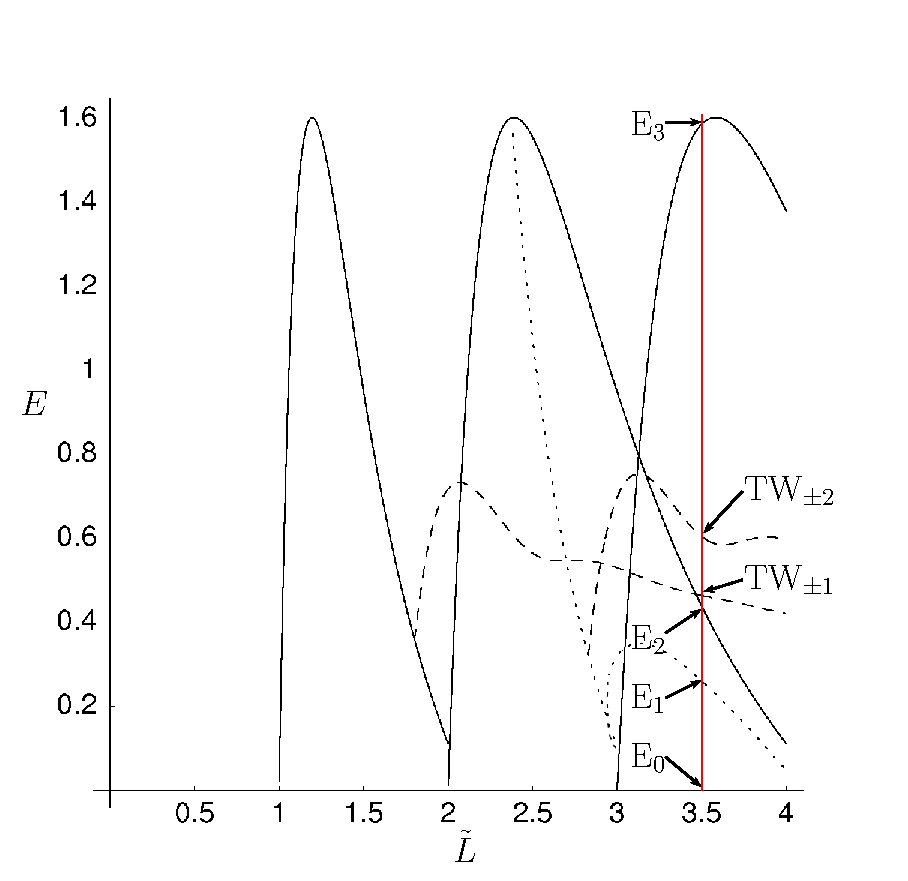
\includegraphics[width=0.5\textwidth]{figs/ksBifDiag_pst.eps}
\end{center}
\caption{
The energy \refeq{ksEnergy} of the \eqva\ and \reqva\ that
exist up to $L=22$, $\tildeL = 3.5014\cdots$, plotted as a function
of the system size $\tildeL = L/2\pi$ (additional \eqva, not present
at $L = 22$ are given in \refref{ksgreene88}). Solid curves denote
$n$-cell solutions \EQV{2} and \EQV{3}, dotted curves the GLMRT
\eqv\ \EQV{1},
% the dash-dotted curve the `giant states' (??? don't have those),
and dashed curves the \reqva\ \REQV{\pm}{1} and \REQV{\pm}{2}.
The parameter $\alpha$ of \refrefs{KNSks90,ksgreene88} is
related to the system size by $\tildeL=\sqrt{\alpha/4}$.
% Open circles indicate Hopf bifurcations.
%The color of a branch indicates the number of unstable eigenvalues:
%(red) 2 unstable eigenvalues, (blue) 1 unstable eigenvalue, (green)
%stable.
        }
\end{figure}
%%%%%%%%%%%%%%%%%%%%%%%%%%%%%%%%%%%%%%%%%%%%%%%%%%%%%%%%%%%%%%%%%%

\ES{Removed text about equilibria of equilibria.}
% ES removed
%%%%%%%%%%%%%%%%%%%%%%%%%%%%%%%%%%%%%%%%%%%%%%%%%%%%%%5
% The solutions of the {\eqv}  condition
% \refeq{eq:3dks} are
% % themselves in turn
% organized\rf{Mks86} by the
% `{\eqva}  of {\eqva}'  condition
% \( u_x= v_x= w_x= 0 \).
% % , and the connections between them.
%     For $\expctE>0$ the {\reqva}  points of \refeq{eqvOfEqv} are
% $C_{+}=(c+\sqrt{2\expctE},0,0)$ and $C_{-}=(c-\sqrt{2\expctE},0,0)$.
% Linearization of the flow around $C_{+}$ yields the cubic equation
% $ %  \beq
% \eigExp(1+\eigExp^2) = 4 \expctE
% \,,
% $ %  \ee{KSeqvCubic}
% with linear stability eigenvalues
% \beq
% \eigExp[1] = 2 \eigRe
%     \,,\qquad
% \eigExp[2,3] = - \eigRe \pm i \eigIm
% \ee{eqvEqvEigV}
% Hence $C_{+}$ has a {1\dmn}
% unstable manifold and a 2\dmn\ stable manifold
% along which solutions spiral in.
% By the $x \to -x$ `time reversal' symmetry, the
% invariant manifolds of $C_{-}$
% have reversed stability properties.
% \PC{
%     not sure we need this, not used in our paper? Where did the figure go?
%     }
% Most orbits escape quickly even if initiated close to \eqva, and that
% renders the numerical calculations
% difficult\rf{ksham95,kshooper88,pimyk,pimsimp}.
% In this context the variational method
% developed in \refrefs{lanVar1,CvitLanCrete02}
% appears more robust than
% the earlier approaches.
%%%%%%%%%%%%%%%%%%%%%%%%%%%%%%%%%%
% end ES removed

%\subsection{\Eqva\ on a periodic domain}
%

%\RLD{This paragraph should probably be moved down after real-space
%equation for equilibria and traveling waves are discussed.}
In the Fourier representation the \reqva\ time
dependence is
\beq
 a_k(t) e^{-itc k/\tildeL} = a_k(0)
\,.
\ee{reqvaF}
Differentiating with respect to time, we obtain
the Fourier space version of the \reqv\ condition
\beq
 \pVeloc_k(a) - i \frac{k c}{\tildeL} a_k = 0
\,,
\ee{reqvCondF}
which we solve for (time independent) $a_k$ and $c$.
Periods of spatially periodic {\eqva} are multiples of $L$.
Every time the system size crosses  $\tildeL=n$,
$n$-cell states
are generated through pitchfork bifurcations off $u =0$
equilibrium.
Due to the translational invariance of {\KSe},
they form invariant circles
in the full \statesp.
In the $\bbU^+$ subspace considered here,
they correspond to $2n$ points, each shifted by $L/2n$.
For a sufficiently small $L$
the number of {\eqva} is small and
concentrated on the low wave-number end of the Fourier spectrum.

In a periodic box of size $L$
both \eqva\ and \reqva\ are  periodic solutions
embedded in 3-$d$ space,
conveniently represented as loops in
$(u,u_x,u_{xx})$ space \ES{dropped 
whose topology is controlled by the
`\eqva\ of \eqva' stable-unstable manifold structure of
\refeq{eqvEqvEigV} }
, see \reffig{f:KS22Equil}\,(\textit{d}).
In this representation the continuous translation symmetry
is automatic - a rotation in the $[0,L]$ periodic domain only
moves the points along the loop. For an \eqv\ the points
are stationary in time; for \reqv\ they move in time, but in
either case, the loop remains invariant.
So we do not have the problem that we encounter in the Fourier
representation, where from the frame of one of the \eqva\
the rest trace out circles under the action of continuous symmetry
translations.


\subsection{Stability of \eqva}
\label{s:StabEqui}
%%
% Predrag           5jun2005
% extracted from \Chapter{stability}{ 2apr2005}

If $u_\stagn(x)$ is an \eqv\ solution of \KSe,
the {\stabmat}
${\Mvar}={\Mvar}(a_\stagn)$
is constant in time,
and
the {\jacobianM}
of the \eqv\ solution is
\beq
 \jMps^t(a_\stagn) = e^{{\Mvar} t}
    \,,\qquad
 \Mvar_{ij}= \Mvar_{ij}(a_\stagn)
\,.
\ee{eqvFundMat}
Calculation of the {\stabmat} requires a bit of care:
% \refeq{DerMatrix}
$a_{k}$ cannot be varied independently of $a_{-k}$, as
% \refeq{expan}
the reality of $u(x,t)$ implies that $a_{k}=a^*_{-k}$.
We impose the reality constraint by splitting \refeq{expan}
in real and imaginary parts, $a_k=b_k+i\, c_k$. {\Stabmat}
is then:
% \index{Kuramoto-Sivashinsky system}
\bea
    \frac{\partial \dot{c}_k}{\partial c_{j}} & = &
    \frac{k^2}{\tildeL^2}\left(1- \frac{k^2}{\tildeL^2} \right)\delta_{kj}
    - \frac{k}{\tildeL} (c_{k+j}-c_{k-j})
\continue
    \frac{\partial \dot{c}_k}{\partial b_{j}} & = &
    - \frac{k}{\tildeL} ( b_{k+j}+b_{k-j} )
\label{expanMvar}\\
    \frac{\partial \dot{b}_k}{\partial b_{j}} & = &
    \frac{k^2}{\tildeL^2}\left(1- \frac{k^2}{\tildeL^2} \right)\delta_{kj}
    +  \frac{k}{\tildeL} (c_{k+j} + c_{k-j})
\continue
    \frac{\partial \dot{b}_k}{\partial c_{j}} & = &
    - \frac{k}{\tildeL} (b_{k+j}-b_{k-j})
    \,,\qquad  k,j>0
\,.
\nnu
\eea
For the \KSe\ the constant solution $u(x,t)=0$ with zero energy $E$ is an
\eqv\ point of \refeq{ks} which we shall henceforth refer to as
\EQV{0}. For this `laminar' \eqv\ the {\stabmat}
is diagonal, and
so is the {\jacobianM}
$
\jMps^t_{kj}(0) = \delta_{kj} e^{(k/\tildeL)^2(1- (k/\tildeL)^2)t}
\,.
$

From \refeq{expan} we see that the origin $u(x,t) = 0$
has Fourier modes as the linear stability eigenvectors.
The $|k|<\tildeL$
long wavelength perturbations of the flat-front {\eqv}
are linearly unstable, while all
$|k|> \tildeL$ short wavelength perturbations are strongly contractive.
The high $k$ eigenvalues, corresponding to rapid variations of
the flame front, decay so fast that the corresponding eigendirections
are physically irrelevant.
The most unstable mode, nearest to $|k|=\tildeL/\sqrt{2}$,
sets the scale of the mean wavelength $\sqrt{2}$
of the KS `turbulent' dynamics,
% measured in the system size \tildeL,
see \reffig{f:ks_largeL}.

\subsection{\Rpo s, symmetries and \po s} \label{sec:KSePO}
% Predrag created file              jul 3 2006

The KS equation \refeq{ks} is time translationally invariant,
and space translationally invariant
under the 1-$d$ Lie group of $O(2)$ rotations: if
$u(x,t)$ is a solution, then $u(x+\shift,t)$ and
$-u(-x+\shift,t)$ are equivalent
solutions for any $-L/2 < \shift \leq L/2$.
As a result, KS can have
%\reqva\ (traveling wave) solutions $u(x-ct)$ and
\rpo\ solutions with period $\period{}$ and
a nonzero shift $\shift$, without or with reflection,
\beq
u(x+\shift,\period{}) = u(x,0)
\,,\qquad \mbox{or } \quad
-u(-x+\shift,\period{}) = u(x,0)
\,,
\ee{KSrpos}
\ie, a profile $u(x,0)$ that occurs again after time $\period{}$,
but shifted by $\shift$, and possibly reflected by $\Refl$.
{\Rpo s} are periodic in $c=\shift/\period{}$
co-rotating frame,
but in the stationary frame their trajectories
are quasiperiodic.
Due to the reflection symmetry \refeq{KSparity} of KS equation,
every {\rpo}
$u(x,t)$ with shift $\shift$ has a symmetric partner
$-u(-x,t)$ with shift $-\shift$.

Our search for \rpo s in KS system were
inspired by Vanessa L{\'o}pez\rf{lop05rel} investigation
of {\rpo s} of the Complex Ginzburg-Landau equation.
However, there is a vast literature on
{\rpo s} since their first appearance,
in  Poincar\'e study of
the 3-body problem\rf{ChencinerLink,rtb} where
the Lagrange points are the \reqva.
They arise in dynamics of systems
with continuous symmetries, such as motions of rigid bodies, gravitational
$N$-body problems, molecules and nonlinear waves.
Very recently Viswanath\rf{Visw07b} % arXiv.org/physics/0604062
has found both \reqva\ and \rpo s in the plane Couette problem.

% PC merged this with \rpo s:
% \subsection{Discrete symmetries imply \po s}

As $\shift$ is continuous in the interval $[-L/2, L/2]$,
the likelihood of a $\shift=0$ shift is zero,
unless an exact periodicity is enforced by a discrete symmetry,
such as the dihedral symmetries discussed above.
If the shift $\shift$ of a \rpo\ with period $\period{}$ is such
that $\shift /L$ is a rational number, then the orbit is
periodic with period $n\period{}$.
Due to the KS equation invariance
under reflection \refeq{KSparity},
two types of \po s are possible:

{\bf (a)} The \po\ lies within the  $\bbU^+$ antisymmetric subspace
$-u(-x,0) = u(x,0)$ and $u(x,\period{}) = u(x,0)$.

{\bf (b)} The \rpo\ in \refeq{KSrpos} is of  reflection type
$\Refl\tau_{\shift/L} u(x,\period{}) = u(x,0)$.
%    \RLD{
%    Maybe we should use symmetry operators throughout the discussion?
%The general idea is that in chaotic systems with symmetries we should
%generalize the notion of a periodic solution from $u(\period{}) = u(0)$
%to $u(\period{}) = {\bf S} u(0)$, where ${\bf S}$ is any symmetry
%a solution of the system might posses.
%\\
%PC: good idea
%    }
In the next period $\period{}$ such orbit
reverses its drift,
$\Refl\tau_{\shift/L} u(-x-\shift,2\period{}) = u(x,0)$, and any
shift acquired during time $0$ to
$\period{}$ is compensated by the opposite shift during
evolution from $\period{}$ to $2\period{}$.
%\[
%u(x,\period{}) = \Refl u(x,\period{}/2) =
%   \Refl^2 u(x,0) = u(x,0)
%   \,.
%\]
\Po s built from repetitions of such shorter segments
are encountered in dynamical systems with discrete
symmetries\rf{CvitaEckardt,DasBuch}.
    \PC{
        are there
        {\bf (c)} \po s which have $D_m$ symmetries?
        }

% history.tex
%
% Predrag created file				jul 3 2006
% $Author$ $Date$


\section{{\Rpo s} - a brief history}

Chenciner\rf{ChencinerLink}
says Poincar\'e introduced them in the 3-body problem.
Consider motion of a test particle of mass
$\mu \ll 1$ in the
restricted three-body problem\rf{rtb},
under the
influence of the gravitational force of two heavy bodies with masses $1$ and
$\mu \ll 1$ fixed at $(-\mu,0)$ and $(1-\mu,0)$. \Reqv\ of this problem
(known in this context as the Lagrange points, stationary in
the co-rotating frame) are circular motions in the inertial frame,
and {\rpo s} correspond to quasiperiodic motions. 

The relative equilibria and relative periodic solutions 
respectively appear from
equilibria and periodic solutions of the Hamiltonian reduced by the symmetries.
They are in many physical situations, which include rigid bodies, gravitational
$N$-body problems, molecules and nonlinear waves.

Lan has some relative equilibria (travelling waves) for KS in his
thesis\rf{Lan:Thesis}, %http://chaosbook.org/projects/theses.html
 and for complex LG in a paper on "MAWs".
Viswanath\rf{ViswanathPC06} % arXiv.org/physics/0604062
found them in the plane Couette problem.
Siminos has for Davidchack box size $L=22$ some equilibria, and all
orbits his \rpo\ search finds are in the set you sent us.

Striking application of \rpo s has been the discovery
of ``choreographies" of $N$-body problems\rf{McC7,McC8,McC}.
\PC{some McCord references}



% L22eqv.tex
%
% Predrag created file              jul  9 2006
% $Author$ $Date$


\section{Small $L=22$ system {\rpo s}}
\label{s:L22}
\file{L22eqv.tex}


\KS\ system with $L = 22$ periodic on the full space is small but
empirically large enough to exhibit persistent chaos.  $L=22$ is a
sensible choice because in units of mean wavelength the size of this
small system is about 2.5 wavelengths ($\tildeL/\sqrt{2}= 2.4758$),
so the dynamics is a competition between wavenumbers 2 and 3.
Because of the strong $k^4$ contraction in \KS\ we expect a small
number of eigenvalues to be significant for the dynamics, while the
rest are in the numerical noise. See figure~6 in
\refref{Christiansen:97}.

%% Davidchack and Crofts
% We investigate this system in 16 to 64 complex Fourier modes (32 to
%128-dimensional system of real ODEs) truncation, and recheck the results
%by redoing the calculation with the double number of Fourier modes. %
%observe how many digits change. The \eqv\ points are accurate to at least
%to $10^{-11}$. Since Lapack is also double precision accurate, the
%accuracy of the first few eigenvalues is similar, and certainly in excess
%of 6 significant digits. % All digits stated in tables are significant.
%The accuracy that can be reached is of order of
%$|a(\period{p},d_p) - a_0|
% \approx \epsilon \exp(\Lyap_p \period{p})$,
% where $\epsilon \approx 10^{-17}$ for double precision, $\Lyap_p$ is
%the largest Lyapunov exponent, and $\period{p}$ the period.  With a good
%starting guess, Newton's method typically reaches that accuracy after 2-3
%iterates.

\subsection{\Eqva}

In addition to the trivial equilibrium $u=0$ (denoted E0 from now
on), we find for $L = 22$ three \eqva\ with dominant wavenumber $k$
(denoted E$k$) for $k = 1, 2, 3$.  All equilibria, shown in
Fig.~\ref{f:KS22Equil}, are symmetric with respect to the reflection
symmetry. The \eqva\ E2 and E3 have additional symmetry with respect
to translation by $L/2$ and $L/3$, respectively.

\begin{figure}[h]\vspace*{-5pt}
\centering
(a)\includegraphics[width=0.25\textwidth]{figs/1wKS22equil.eps}
(b)\includegraphics[width=0.25\textwidth]{figs/2wKS22equil.eps}
(c)\includegraphics[width=0.25\textwidth]{figs/3wKS22equil.eps}
\vspace*{-5pt}\caption{ {\small (a) E1, (b) E2 and (c)
E3~\eqva\ of \KS\ equation with $L=22$.}}
\label{f:KS22Equil}\vspace*{-5pt}
\end{figure}

%\begin{figure}
%  \includegraphics[width=12cm]{figs/L22-E123.eps}\\
%  \caption{\KSe\ equilibria for $L=22$.}\label{fig:E123}
%\end{figure}

The stability of the equilibria is characterized by the eigenvalues
$\lambda_j$ of the Jacobian matrix.  First ten eigenvalues for each
equilibrium are listed in Table~\ref{tab:Ek_eigs} in the order of
decreasing real parts. Recall that an equilibrium with $\mathrm{Re}
\lambda_j > 0$ is unstable in the direction of the corresponding
eigenvector $e_j$.

\begin{table}
\caption{\label{tab:Ek_eigs} Eigenvalues of the \eqva\ for $L=22$.}
{\small
\begin{tabular}{cccc} \hline
  E0       &        E1         &         E2        &     E3   \\\hline
  $0.2198$ &  $0.1308+i0.3341$ &  $0.1390+i0.2384$ &  $0.0933$\\
  $0.2198$ &  $0.1308-i0.3341$ &  $0.1390-i0.2384$ &  $0.0933$\\
  $0.1952$ &  $0.0824+i0.3402$ &  $0$              &  $0$\\
  $0.1952$ &  $0.0824-i0.3402$ & $-0.0840+i0.1602$ & $-0.4128$\\
  $0.0749$ &  $0$              & $-0.0840-i0.1602$ & $-0.6108+i0.3759$\\
  $0.0749$ & $-0.2287+i0.1963$ & $-0.1194$         & $-0.6108-i0.3759$\\
 $-0.3981$ & $-0.2287-i0.1963$ & $-0.2711+i0.3563$ & $-0.6108+i0.3759$\\
 $-0.3981$ & $-0.2455$         & $-0.2711-i0.3563$ & $-0.6108-i0.3759$\\
 $-2.1191$ & $-2.0554$         & $-2.0130$         & $-1.6641$\\
 $-2.1191$ & $-2.0619$         & $-2.0378$         & $-1.6641$\\\hline
\end{tabular}}
\end{table}

The eigenvalues of E0 are determined by the linear part of the \KS\
equation: $\lambda_k=q_k^2-q_k^4$, where $q_k = 2\pi k/L$.  For
$L=22$, there are three pairs of unstable eigenvalues: corresponding
to three unstable modes $k=2,3$, and 1, respectively.  For each
mode, the corresponding eigenvectors lie in the plane spanned by
$\mathrm{Re} a_k$ and $\mathrm{Im} a_k$. Tables \ref{tab:E1_sym} to \ref{tab:E3_sym}
list the symmetries corresponding to the stability eigenvectors of \eqva E1-E3.
With $S$, $A$ we denote an eigenvector belonging to the symmetric
or antisymmetric subspace respectively. The last column lists
the symmetry expected to be present in the corresponding
stable/ustable manifold.

\begin{table}[h!]
\caption{\label{tab:E1_sym} Symmetries of eigenvectors of E1 for $L=22$.}
{\small
\begin{tabular}{cccc} \hline
          $\lambda_i$       & $\mathrm{Re}(e_i)$    & $\mathrm{Im}(e_i)$    & $\mathcal{M}$ \\\hline
    $0.1308 \pm i0.3341$    & S     & S     & - \\
    $0.0824 \pm i0.3402$    & A     & A     & A \\
    $0$                     & S     &       & - \\
    $-0.2287+i0.1963$       & A     & A     & A \\
    $-0.2455$               & S     &       & - \\
    $-2.0554$               & A     &       & A \\
    $-2.0619$               & S     &       & - \\\hline
\end{tabular}}
\end{table}

\begin{table}[h!]
\caption{\label{tab:E2_sym} Symmetries of eigenvectors of E2 for $L=22$.}
{\small
\begin{tabular}{cccc} \hline
          $\lambda_i$       & $\mathrm{Re}(e_i)$    & $\mathrm{Im}(e_i)$    & $\mathcal{M}$ \\\hline
      $0.1390\pm i0.2384$   & A     & A     & A \\
      $0$                   & S     &       & - \\
      $-0.0840\pm i0.1602$  & S     & S     & - \\
      $-0.1194$             & S     &       & - \\
      $-0.2711\pm i0.3563$  & A     & A     & A \\
      $-2.0130$             & S     &       & - \\
      $-2.0378$             & A     &       & A \\\hline
\end{tabular}}
\end{table}

\begin{table}[h!]
\caption{\label{tab:E3_sym} Symmetries of eigenvectors of E3 for $L=22$.}
{\small
\begin{tabular}{cccc} \hline
          $\lambda_i$    & $\mathrm{Re}(e_i)$    & $\mathrm{Im}(e_i)$    & $\mathcal{M}$ \\\hline
    $0.0933$             &  A    &       & A \\
    $0.0933$             &  S    &       & - \\
    $0$                  &  S    &       & - \\
    $-0.4128$            &  A    &       & A \\
    $-0.6108\pm i0.3759$ &  A    &   A   & A \\
    $-0.6108\pm i0.3759$ &  S    &   S   & - \\
    $-1.6641$            &  S    &       & - \\\hline
\end{tabular}}
\end{table}


\subsection{Unstable invariant manifolds of \eqva\ and heteroclinic
connections}

In this section we explore the structure of unstable invariant
manifolds of the equilibria.  The E1 equilibrium has two unstable
planes within which the solutions are spiralling out (i.e., two
pairs of complex conjugate eigenvalues).  The E2 has one such plane,
while the E3 has two real positive eigenvalues, so the solutions are
moving radially away from the equilibrium within the plane spanned
by the corresponding eigenvectors.  Since E1 has larger unstable
subspace, it is expected to have much less influence on the system
evolution compared to E2 and E3.

\begin{figure}[h]\vspace*{-5pt} \centering
\includegraphics[width=0.45\textwidth]{figs/ks22_E1_plane1_manifold.eps}
\includegraphics[width=0.3\textwidth]{figs/ks22_E1_plane1_orbits.eps}
\vspace*{-5pt}\caption{ {\small The upper panel shows the unstable
invariant manifold of equilibrium E1 starting within the plane
corresponding to the first pair on unstable eigenvalues. The
coordinate axes $v_1$, $v_2$, and $v_3$ are constructed from vectors
$\mathrm{Re} e_1$, $\mathrm{Im} e_1$, and $\mathrm{Re} e_6$
by Gram-Schmidt orthogonalization.
The lower panel shows spacial representation of two orbits A and B.
The change of color from blue to red indicates increasing values of
$u(x)$.}} \label{f:KS22E1man1}\vspace*{-5pt}
\end{figure}

To construct an invariant manifold containing solutions
corresponding to the pair of unstable complex conjugate eigenvalues,
$\lambda = \sigma\pm i\omega$, $\sigma > 0$, we start with a set of
initial conditions near equilibrium $a_{\mathrm{E}k}$:
\[ a(0) = a_{\mathrm{E}k} + \epsilon\,v\mathrm{e}^{\delta}\]
where $\delta$ takes the set of values uniformly distributed in the
interval $[0,2\pi\sigma/\omega]$, $v$ is a unit vector in the
unstable invariant plane, and $\epsilon > 0$ is small.

\begin{figure}[h]\vspace*{-5pt} \centering
\includegraphics[width=0.45\textwidth]{figs/ks22_E1_plane2_manifold.eps}
\includegraphics[width=0.45\textwidth]{figs/ks22_E1_plane2_orbits.eps}
\vspace*{-5pt}\caption{ {\small The upper panel shows the unstable
invariant manifold of equilibrium E1 starting within the plane
corresponding to the second pair on unstable eigenvalues. The
coordinate axes $v_1$, $v_2$, and $v_3$ are constructed from vectors
Re $e_3$, Im $e_3$, and Re $e_6$ by Gram-Schmidt orthogonalization.
The lower panel shows spacial representation of three orbits. Orbits
B and C pass close to the equilibrium E3.}}
\label{f:KS22E1man2}\vspace*{-5pt}
\end{figure}

The manifold starting within the first unstable plane of E1, with
eigenvalues $0.1308\pm i0.3341$, is shown in
Figure~\ref{f:KS22E1man1}. It appears to fall directly into the
chaotic attractor.  The behaviour of the manifold starting within
the second unstable plane of E1 (eigenvalues $0.0824\pm i0.3402$) is
remarkably different: as can be seen in Figure~\ref{f:KS22E1man2},
all orbits within the manifold converge to the equilibrium E2.  The
manifold also contains a heteroclinic connection from E1 to E3.

\begin{figure}[h]\vspace*{-5pt} \centering
\includegraphics[width=0.45\textwidth]{figs/ks22_E2_manifold.eps}
\includegraphics[width=0.45\textwidth]{figs/ks22_E2_orbits.eps}
\vspace*{-5pt}\caption{ {\small The upper panel shows the two-dimensional
unstable invariant manifold of equilibrium E2. The coordinate axes
$v_1$, $v_2$, and $v_3$ are constructed from vectors
Re $e_1$, Im $e_1$, and $e_7$ by Gram-Schmidt orthogonalization.
The lower panel shows spacial representation of three orbits. Orbits
B and C pass close to the equilibrium E3.}}
\label{f:KS22E2man}\vspace*{-5pt}
\end{figure}

The two-dimensional unstable manifold of E2 is shown in
Figure~\ref{f:KS22E2man}.  All orbits within the manifold converge
to E2 shifted by $L/4$.  So this manifold can be viewed as a homoclinic
connection.  It also contains a pair of heteroclinic connections from
E2 to E3.

The equilibrium E3 has a pair of real unstable eigenvalues
equal to each other.  Therefore, within the plane spanned by the
corresponding eigenvectors, the orbits move radially away from
the equilibrium.  In order to trace out the unstable manifold,
we start with a set of initial conditions within the unstable plane
\[ a(0) = a_\mathrm{E3} + \epsilon(v_1 \cos \phi + v_2 \sin \phi)\,,
  \quad\phi\in[0,2\pi]\,, \]
where $v_1$ and $v_2$ are orthonormal vectors within the
plane spanned by the two unstable eigenvectors.  The unstable manifold
of E3 is shown in Figure~\ref{f:KS22E3man}.  The 3-fold symmetry of
the manifold is related to the symmetry of E3 with respect to
translation by $L/3$.  The manifold contains heteroclinic orbits
connecting E3 to three different points of the continuum of equilibria E2
translated by 0 and $\pm L/6$.  Note that there are two different
heteroclinic orbits (B and C) connecting E3 to the same point in the E2
continuum.  Note also that the segments of orbits B and C
between E3 and E2 in Figures~\ref{f:KS22E1man1} and \ref{f:KS22E2man}
represent the same heteroclinic connections as orbits B and C in
Figure~\ref{f:KS22E3man}.

\begin{figure}[h]\vspace*{-5pt} \centering
\includegraphics[width=0.4\textwidth]{figs/ks22_E3_manifold.eps}
\includegraphics[width=0.45\textwidth]{figs/ks22_E3_orbits.eps}
\vspace*{-5pt}\caption{ {\small The upper panel shows the two-dimensional
unstable invariant manifold of equilibrium E2. The coordinate axes
$v_1$, $v_2$, and $v_3$ are constructed from vectors
$e_1$, $e_2$, and $e_4$ by Gram-Schmidt orthogonalization.
The black line shows a family of E2 equilibria related by translational
symmetry The lower panel shows spacial representation of
three orbits. Orbits B and C are two different heteroclinic orbits
connecting E3 to the same point on the E2 line.}}
\label{f:KS22E3man}\vspace*{-5pt}
\end{figure}



The unstable manifold plane is traced out in
\reffig{f:neighborhood2w}(a). Computed the 2 expanding eigenvectors
of the \eqv\ {\nameit}2, as well as the 3rd, least contracting
direction; then translated and rotated Fourier modes into this
coordinate frame, plotted the unstable manifold.
% trajectory there, both in the lab and the mean velocity frame.


 It is the unstable manifold of the \nameit 2
{\eqv}, drawn by tracing out a set of points along one of the complex
eigenvectors, that start close to it. Surprisingly, everybody connects
to the \nameit 2 shifts by 1/2 wavelength (d = L/4 = 5.5) but as we are in
infty dimensions they do it not as the usual homoclinic connection, but in
many (all?) possible intermediate ways. This might be a clue for how to
partition symbolic dynamics. Note also that in your L22-long.eps one seems
to come quite close to \nameit 2 {\eqv}, so it might be a very dominant
influence on the strange attractor dynamics


There appears to be a heteroclinic connection from \nameit 2
{\eqv}
unstable spiral out straight into \nameit 3 {\eqv}
$\period{} = 76.6$ \rpo\ seems like a closeby
relative of this.
That also means that the relative shift between the two {\eqva} is
fixed, as far as this connection is concerned.

What is great about
this is that the \nameit 2 unstable manifold has a heteroclinic connection to itself
$L/2$ shifted, but
even better, to \nameit 2, and \nameit 3 unstable manifold has a heteroclinic
connection to \nameit 2.
It's really pretty. That makes for a rigid backbone -
we hope this will help us develop a symbolic dynamics for rpo's.

It is very unlikely that a single 1-$d$ Poincar\'e section,
can do the job, previous work\rf{Lan:Thesis,LanCvi06}
always needed several sections.

The idea is that the local unstable plane gives 2 coordinates, the
least contracting direction (or one of a complex pair) gives the 3rd.

We need to construct the backbone of heteroclinic connections
first. They are not like 3-$d$ R\"ossler and Lorenz examples:
here one spirals out,
then spirals in - hopefully there will be intelligent Poincar\'e sections
transverse to initial \nameit 2 (or \nameit 3) unstable manifold, mapping onto
Poincar\'e sections of trajectories leaving again
the next \nameit 3 or \nameit 2 unstable manifold.


Check next what these 2 unstable eigenvectors for \nameit 3 eqv. are - when they
are equal in magnitude you expect a `star', all directions in their plane
going straight out. Do they all fall int \nameit 2 eqv?

% Ruslan:  10 Jul 2006
%
% 119 KB     "long_orbit.jpg"
%  88 KB     "steady_states1.jpg"
%  84 KB     "steady_states2.jpg"
% 197 KB     "rpos1.jpg"
% ----------------------------------------

For all spatial plots color axis $u \in [-3, 3]$ is the same,
same time units and spatial width $L$.
For the steady states the magnitude of the \nameit 2 is quite
a bit smaller than that of the \nameit 3.

On the
    $[a_?,a_?]$ plane
    the $\sigma x = -x$ symmetry of \KSe\ is explicit.


steady\_states1.jpg shows the numerical evolution and, since the
traveling wave is very unstable, it disappears after awhile.
The numerically exact solution is plotted in steady\_states2.jpg

rpos1.jpg is attached as a sample.

As it looks, will not help us with partitioning, it seems, unless there is
a trajectory that hits the contracting direction - maybe
( -0.11941393,0)
head on.

Might want to look at this blowup in
the \nameit 2 slowest contraction
$   ( -0.08402656 \pm i 0.16019413)$
complex eigenvectors plane, check whether the
spiralling rotation agrees with the real/imaginary parts of eigenvalues.

Question is still - why does all of the unstable manifold of
\nameit 2 \eqv\ go back
into
\nameit 2 \eqv ?

%%%%%%%%%%%%%%%%%%%%%%%%%%%%%%%%%%%%%%%%%%%%%%%%%%%%%%%%%%%%%%%%
\begin{figure}[h]
\centering
(a) 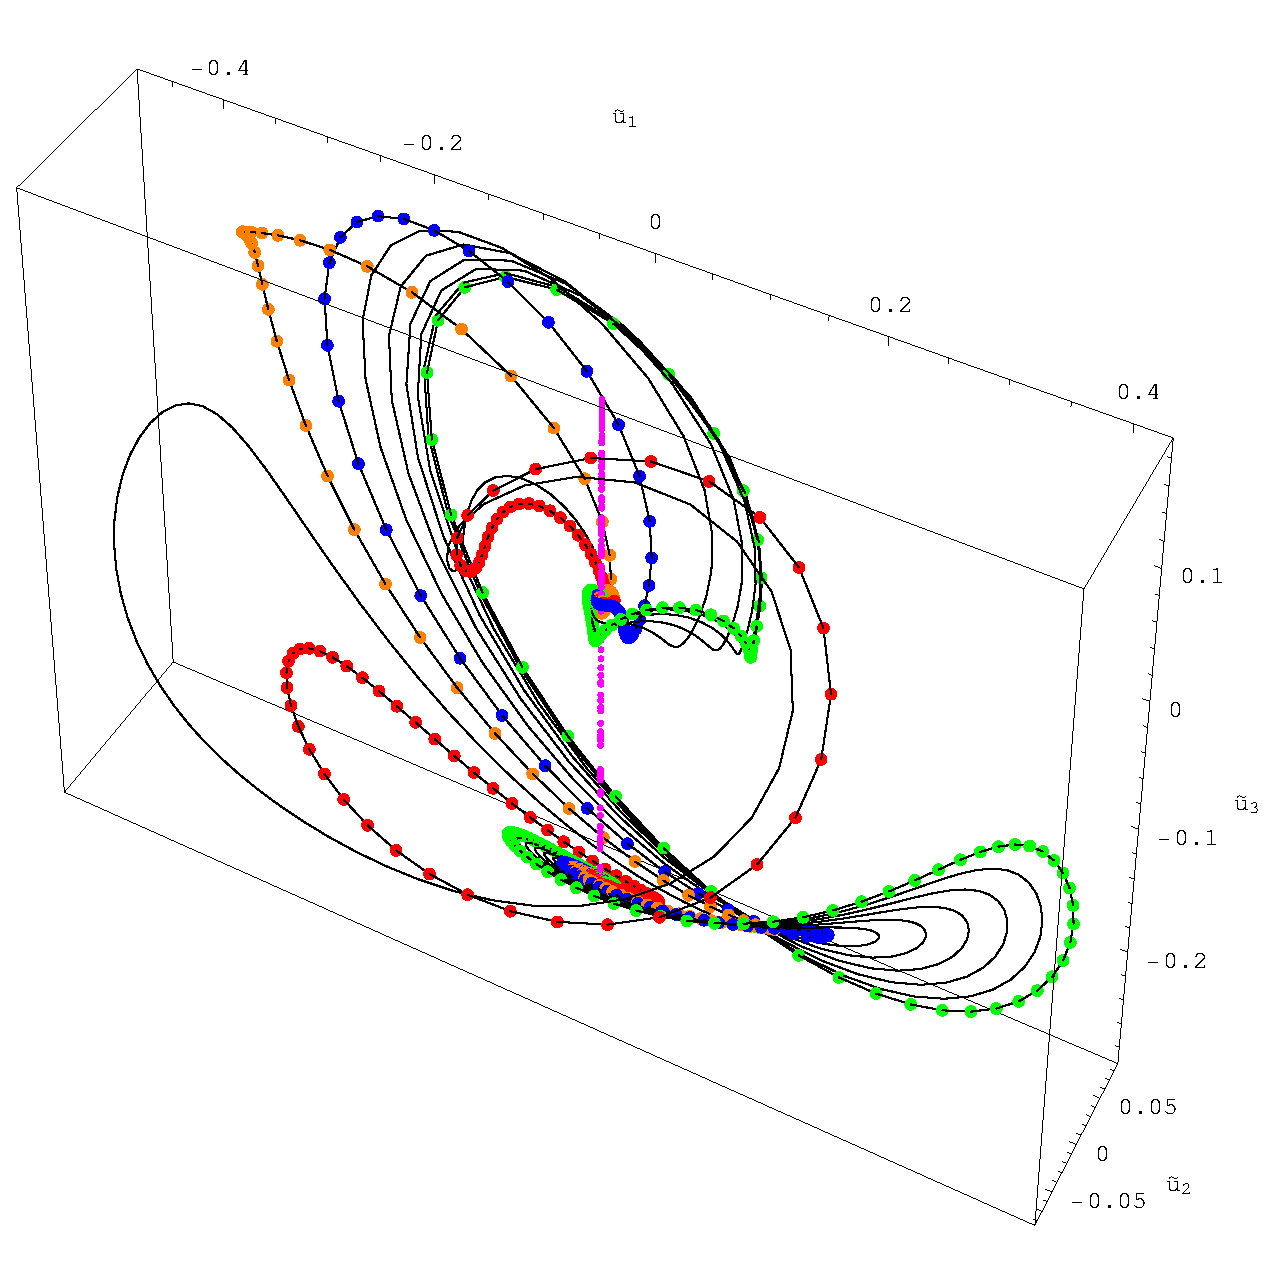
\includegraphics[width=5.0cm]{figs/L22-2w-UnsMan.eps}
\hspace{0.1in}
(b) \includegraphics[width=5.0cm]{figs/L22-2w-UnsMan-BlowUp.eps}
% (b) \includegraphics[width=4.0cm]{figs/L22-2w-R.eps}
\\
(c) \includegraphics[width=5.0cm]{figs/L22-2w-3w-UnsMan.eps}
% (c) \includegraphics[width=4.0cm]{figs/L22-2w-G.eps}
\hspace{0.1in}
(d)  \includegraphics[width=5.0cm]{figs/L22-2w-3w-detail.eps}
% (d) \includegraphics[width=4.0cm]{figs/L22-2w-B.eps}
\caption{
 Trajectories with initial conditions on the unstable subspace of
 the \nameit 2 {\eqva}.
 (a) The coordinates $\tilde{u}_1$ and $\tilde{u}_2$ are along the directions defining the unstable subspace
 and $\tilde{u}_3$  is along the real part of the eigenvector,
 corresponding to the eigenvalue $-0.271122+ i\, 0.356307$. The purple points represent the continous family
 of
\nameit 2 \eqva.
% Green curve belongs to \reffig{f:rpo55}(b) % rpo22-55-4-cm.eps
% rather than to  \reffig{f:rpo55}(a), % rpoEq22-55-4.eps?
(b) blowup of ``homoclinic'' descent of the unstable manifold
back into {\nameit}-2 {\eqv}, shifted by
$L/4 =5.5$.
(c) blowup of ``heteroclinc'' connection from
{\nameit}2 \eqv\ to {\nameit}3 \eqv\, with shift
$L(1/3-1/4) = L/12 = 1.83$ (? check)
to the neighborhood of the point near which the
unstable manifold of the
\nameit 2 \eqv\ splits. The blue points
represent the
\nameit 3 {\eqv} family.
The descent is along the eigenvector of $\Lyap_4= 0.413$ (checked by ES),
and spliting
occurs along one of the
$\Lyap_1=\Lyap_2=0.0933$
unstable directions of the \nameit 2 {\eqv} (checked by ES).
d) same as (c), closer to the \nameit 3 {\eqv}. The eigendirections corresponding to $\Lyap_1$
and $\Lyap_4$ are shown in purple.
}
\label{f:neighborhood2w}
\end{figure}
%%%%%%%%%%%%%%%%%%%%%%%%%%%%%%%%%%%%%%%%%%%%%%%%%%%%%%%%%%%%%%%%%%


\subsection{\Reqva}

In addition to the \eqva\ , the \KS\ system has \reqv\ solutions
(also called traveling or rotating waves in the literature).
They are characterized by a fixed function profile, $u(x)$,
moving with constant speed $c$, i.e.
\[ u(x+ct,t) = u(x, 0)\,,\quad t \in \mathbb{R}\,.\]
Because of the reflection symmetry, the \reqva\ come in pairs
related by the transformation: $u(x) \to -u(-x)$, $c \to -c$.
In Fourier space the \reqva\ are defined by the condition
\[ a_k(t)\mathrm{e}^{-iq_kct} = a_k(0)\,.\]
Differentiating this condition with respect to time, we obtain
equation for the \reqv\
\[ f_k(a) - i q_k c a_k = 0 \]
which needs to be solved for $a_k$ and $c$.

Consistent with the bifurcation diagram of Greene and Kim,
we find two \reqva\ with speeds $c = 0.737$ and $0.350$.
The profiles of the two \reqva\ and their time evolution
with eventual fall into the chaotic attractor are
shown in Figure~\ref{f:ks22tw}.


\underline{1-\reqv\  (traveling wave).}
% Ruslan L Davidchack,  10 Jul 2006
There is a pair of \reqva\
${\nameit}1L$,
${\nameit}1R$
(traveling waves), dual under the
$u(x) \to -u(-x)$ symmetry. They are
determined numerically by
adiabatic continuation from a smaller system size
$L~\approx 12$,
where they are stable, to $L=22$
where their velocity is atypically large, $c=0.737$,

Their exponents are:
\\
$\Lyap_i \pm \theta_i =
(
\\
  0.1156222 \pm 0.817289,   \\
  0.033663 \pm 0.418909,    \\
 0.0                    ,   \\
 -0.245729                    , \\
 -0.321321 \pm 0.98126,
\cdots
)$

The pair of \reqva\
${\nameit}2L$,
${\nameit}2R$
exists for larger system sizes, but does not continue
adiabatically\rf{KNSks90} down to $L=22$.


\subsection{\Eqva, $L$ and $c$}

%%%%%%%%%%%%%%%%%%%%%%%%%%%%%%%%%%%%%%%%%%%%%%%%%%%%%%%%%%%%%%%%
\begin{figure}[t]
    % \vspace*{-5pt}
\centering
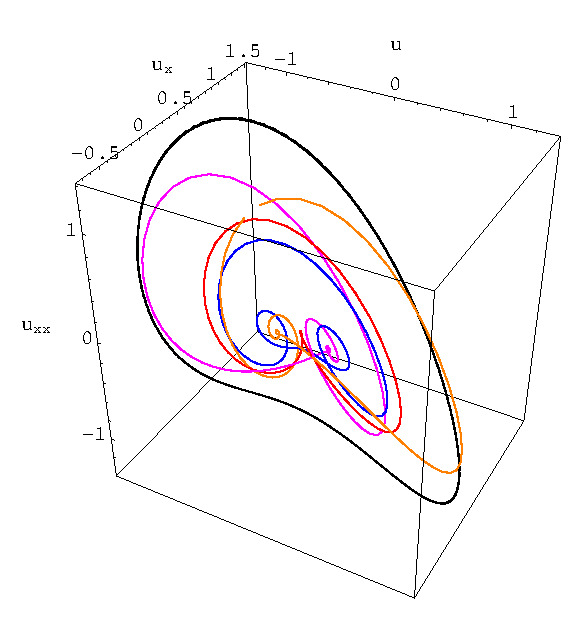
\includegraphics[width=0.6\textwidth]{figs/equilSpatial.eps}
    % \vspace*{-5pt}
\caption{
    {\small
$(u,u_x,u_{xx})$ representation
of $\EQV{1}$ (blue), $\EQV{2}$ (red), $\EQV{3}$ (black) \eqva\ and $\REQV{+}{1}$ (purple), $\REQV{-}{1}$ (orange) \reqva.
$\tildeL=3.5014$, $N=64$ complex modes truncation.
        } %end \small
        }
\label{f:eqvSpatial}
    % \vspace*{-5pt}
\end{figure}
%%%%%%%%%%%%%%%%%%%%%%%%%%%%%%%%%%%%%%%%%%%%%%%%%%%%%%%%%%%%%%%%%%

\PC{
 add the left/right $\REQV{\pm}{1}$ pair to \reffig{f:eqvSpatial}
    }
The $u=0$  \eqv\ $\EQV{0}$ is a point at the origin
in \reffig{f:eqvSpatial}.
At
each integer value of $\tildeL$ the origin spews out a Hopf cycle. That
might help us prove that we have all equilibria for $L=22$.

Each of these \eqva\ has a different value of the $c$ integration
constant.

Plot also the two \eqva\ of \eqva\ points, their
real eigenvectors and their complex eigenplanes. All equilibria presumably
wind around these, and as box size $L$ changes, they form continuous
families with smoothly changing $c$. One can check that by
changing $L$ a bit and using the previous equilibrium to find the next
one.

What does the complex eigenplane continuation does for these
equilibria - does it produce nice heteroclinic connections, or is it
wierder? We know there is an analytic formula for a heteroclinic
connection (see \refref{Lan:Thesis}). % Lan's thesis).

The real motivation for all this is that if we understand \eqva\ as
$L \to \infty$ we might have an entry into $L = \infty$ periodic orbit
theory of KS.

%%%%%%%%%%%%%%%%%%%%%%%%%%%%%%%%%%%%%%%%%%%%%%%%%%%%%%%%%%%%%%%%
\begin{figure}[h]
\centering
(a) \includegraphics[width=5.0cm]{figs/1wSteadyE.eps}
\hspace{0.1in}
(b) \includegraphics[width=5.0cm]{figs/1wSteadyP.eps}
\caption{
\small{
(a) $\EQV{1}$ in $(u,u_x,u_{xx})$ representation along with the eigenvectors of the equilibrium
point $(\sqrt{c},0,0)$. The blue line represents the unstable eigen-direction.
(b) $\EQV{1}$ projected along the above eigenvectors. $\tildeL=3.5014$, $N=64$ complex modes truncation.
}
}
\label{f:1wSteady}
\end{figure}

\reftab{tab:L22cminus} lists the stability eigenvalues
$\eigExp[1]^-,\eigRe[2]^-\pm\eigIm[2]^-$
of equilibrium point $c_{-}=(-\sqrt{c},0,0)$
of \label{eq:3dks} for $c$ corresponding to each on of $\EQV{1},\EQV{2}$ and $\EQV{3}$ \eqva.
The period of spiraling $T_{-}=2\pi/\theta^-_2$, expansion
rate in the complex plane of spiraling
$\ExpaEig_r\approx\exp(\eigRe[2]^- T_-)$ and contraction
rate along the stable eigendirection
$\ExpaEig_1\approx\exp(\eigRe[1]^- T_-)$ are also listed.

\begin{table}[h!]
% use packages: array
    \begin{tabular}{l|rrrrrr}
                & $E$   &$\eigExp[1]^-$ & $\eigRe[2]^-\pm\eigIm[2]^-$   & $T_m$ & $\ExpaEig_r$  & $\ExpaEig_1$  \\ \hline
        $\EQV{1}\ $ &\ 0.13 &\ -0.55    &\ $0.28\pm1.11i$       &\ 5.67     &\ 4.79     &\ 0.04 \\ \hline
        $\EQV{2}\ $     &\ 0.22 &\ -0.66    &\ $0.33\pm1.15i$       &\ 5.47     &\ 5.99     &\ 0.03 \\ \hline
        $\EQV{3}\ $     &\ 0.79 &\ -0.94    &\ $0.47\pm1.29i$       &\ 4.87     &\ 9.92     &\ 0.01
    \end{tabular}
    \caption{}
    \label{tab:L22cminus}
\end{table}


%%%%%%%%%%%%%%%%%%%%%%%%%%%%%%%%%%%%%%%%%%%%%%%%%%%%%%%%%%%%%%%%%%

% relativeKS.tex
% copied here from nsf/nsf06am/TEX/relativeKS.tex       Nov 1 2006
% $Author$ $Date$


\subsection{\Eqva}

The KS work
% described in \refsect{s:KS}
of \refref{Christiansen:97}
was restricted to the antisymmetric subspace.
The restriction to antisymmetric subspace was used
to eliminate the continuous translational symmetry of \KSe.
Due to the lack of self-adjointness
(non-normality) of the linearized \KS\ flow, 
the antisymmetric subspace
is unstable under small perturbations, and generic solutions of 
KS belong to the full, periodic space.
Nevertheless, 
the \eqva\ and the shortest \po s orbits that lie in this subspace
and play important role for global topology of the flow,
together
with the \reqva\ and \rpo s
characteristic of the full, continuous translation invariant space..
%%%%%%%%%%%%%%%%%%%%%%%%%%%%%%%%%%%%%%%%%%%%%%%%%%%%%%%%%%%%%%%%
\begin{figure}[t]
\begin{center} 
(a) %\includegraphics[width=0.33\textwidth]{figs/kse22_E1_UM2.eps}
~~~
(b)\includegraphics[width=0.3\textwidth]%,origin=c]%
        {figs/ks22E2-E3hetero.ps}
\end{center}
\caption{OBSOLETE:
(a) \EQV{1}~\eqv\ unstable manifold, 
    with the trajectory connecting the
\EQV{2}~\eqv\ point to the unique corresponding heteroclinic
point in the \EQV{3}~\eqv\ family. 
\EQV{3}~unstable manifold in turn connects \EQV{3} to the
stable manifold of \EQV{2}.
(b) \EQV{2}~\eqv\ to \EQV{3}~\eqv\ heteroclinic 
connection. Here we omit the unstable manifold of \EQV{2},
keeping only a few neighboring trajectories in order to indicate
the unstable manifold of \EQV{3}, and show the \EQV{2} and \EQV{3}
families of \eqva\ arising from the continuous translational
symmetry of KS on a periodic domain. 
% separatrix.
% $\tilde{L}=3.5014$, 2$d$ projections from 64 
% complex Fourier modes \statesp.
        }
\label{f:KS22unstM}
\end{figure}
%%%%%%%%%%%%%%%%%%%%%%%%%%%%%%%%%%%%%%%%%%%%%%%%%%%%%%%%%%%%%%%%%%
\PC{a bit of a cheat - \reffig{f:KS22unstM} has
    2 unstable complex-pair planes}

In \reffig{f:KS22unstM}(b) the \eqv~\EQV{1} of
\reffig{f:KS22unstM}(a) is represented by the point~\EQV{1},
and its unstable manifold can be examined in great detail.
To each \eqv\ point corresponds a continuous family
of \eqva, and this leads to an unexpected feature of such
flows: While in dimensions higher than 2 heteroclinic connections 
are a rarity (likelihood that unstable manifold of one
 \eqv\ precisely hits another \eqv\ point is zero), 
for flows with continuous symmetries intersections of unstable
manifolds with continuous families of equivalent \eqva\ are common.
\refFig{f:KS22unstM}(b) and (c) show 
such heteroclinic connections.
% from an $\EQV{2}$~\eqv\ point to $\EQV{3}$~\eqv\ family.
These connections partition the \statesp,
and will be the basis of our
{\bf construction of symbolic dynamics}.
Effective symbolic dynamics allows
for a systematic and exhaustive determination 
of all \rpo s, in the spirit of 
the earlier work. \PC{refer to it}
Many short unstable \rpo s have been already 
been computed using trial trajectories based on above
topological connections as starting  guesses 
for variants of the Newton method.


%%%%%%%%%%%%%%%%%%%%%%%%%%%%%%%%%%%%%%%%%%%%%%%%%%%%%%%%%%%%%%%%
\begin{figure}[t]
\begin{center} 
%\includegraphics[width=0.6\textwidth]{figs/ks22manifold.ps}

\includegraphics[height=2in]{figs/ks22manifold1.eps}
\end{center}
\caption{
    Unstable manifold of \EQV{2}~\eqv.
%\ of KS equation for $\tilde{L}=3.5014$, N=64 mode truncation.
    (black line) the family of \EQV{2}~\eqva\ 
obtained by application of the translation operator. 
(purple line) the family of \EQV{3}~\eqva.
(red) the heteroclinic connection 
from the \EQV{2}~\eqv\ to the \EQV{3}~\eqv.
The connection splits the manifold into two parts, 
colored blue and green here.
        }
\label{f:KS22Manifold}\vspace*{-5pt}
\end{figure}
%%%%%%%%%%%%%%%%%%%%%%%%%%%%%%%%%%%%%%%%%%%%%%%%%%%%%%%%%%%%%%%%%%


%%%%%%%%%%%%%%%%%%%%%%%%%%%%%%%%%%%%%%%%%%%%%%%%%%%%%%%%%%%%%%%%
\begin{figure}[t] \label{f:KS22rpo}
\begin{center} 
(a)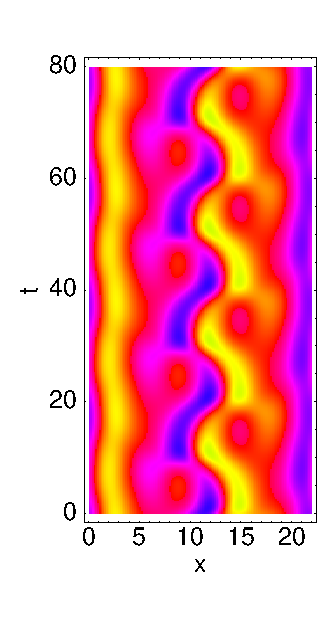
\includegraphics[width=0.2\textwidth]{figs/rpoKS21.eps}
(b)\includegraphics[width=0.2\textwidth]%,origin=c]
                {figs/rpoKS33.eps}
(c)\includegraphics[width=0.2\textwidth]%,origin=c]%
        {figs/rpoKS46.eps}
(d)\includegraphics[width=0.2\textwidth]%,origin=c]%
        {figs/rpoKS56.eps}
\end{center}
\caption{
\Rpo s of KS
equation:
% for $\tilde{L}=3.5014$, N=64 mode truncation.
(a) T=20.51, d=0.0 (\po),
(b) T=32.80, d=10.96,
(c) T=46.51, d=7.76,
(d) T=55.60, d=-5.25.
        }
\end{figure}
%%%%%%%%%%%%%%%%%%%%%%%%%%%%%%%%%%%%%%%%%%%%%%%%%%%%%%%%%%%%%%%%%%




% newton.tex
%
% Predrag			jun 20 2006
% Vaggelis			may 20 2006
% $Author$ $Date$


% \section{Newton's method for determining \reqva}
% 
%  Our task is to find \reqva\ solutions of \refeq{eq:KS}.
% Although one can easilly see that this problem can be reduced to that of
%  finding periodic orbits of a 4-dimensional ODE, here we prefer to consider our system in phase space and search for solutions of
%  \beq
% 	\dot{b}_k=\dot{c}_k=0\,,
%  \eeq
%  for every $k$. The reason to do this is just getting experience before pursuing the more difficult task of locating POs and RPOs. 
%  Expanding $\dot{b}_k(a)$ and $\dot{c}_k(a)$ around our initial guess $a_o$ and demanding that they satisfy the equilibrium 
%  condition, we get
%  \bea
% 	\dot{b}_k(a) & = & \dot{b}_k(a_o)+\left.\frac{\partial \dot{b}_k}{\partial b_j}\right|_{a_o}\delta b_j + \left.\frac{\partial \dot{b}_k}{\partial c_j}\right|_{a_o}\delta c_j = 0 \continue
% 	\dot{c}_k(a) & = & \dot{c}_k(a_o)+\left.\frac{\partial \dot{c}_k}{\partial b_j}\right|_{a_o}\delta b_j + \left.\frac{\partial \dot{c}_k}{\partial c_j}\right|_{a_o}\delta c_j = 0
%  \eea
%  or in matrix form
%  \beq
%     \left( \begin{array}{cc}
%         \frac{\partial \dot{b}}{\partial b} & \frac{\partial \dot{b}}{\partial c} \\
%         \frac{\partial \dot{c}}{\partial b}	& \frac{\partial \dot{c}}{\partial c}
%      \end{array}
%      \right)_{a_o}
%      \left(\begin{array}{c}
%        \delta b  \\
%        \delta c
%      \end{array}\right)
%      =
%      \left(\begin{array}{c}
%        -\dot{b}(a_o) \\
%        -\dot{c}(a_o)
%      \end{array}\right)\,,
%      \label{eq:NewtonEquil}
% \eeq
% where $\partial{\dot{b}} / \partial{b}$ \etc are $d \times d$ submatrices. Solving this
% system of equations for the corrections $\delta b$ and  $\delta c$ and using the refined solution
% as an initial guess yields  an approximation to the solution of the system.
%  


\subsection{Implementing Newton's method  for RPOs}
\label{sec:NewtRPOs}

The relative periodic condition
\beq
	u(x+d,t+T)=u(x,t) \,
\eeq
translates in Fourier space into
\beq	
	\sum_{k=-\infty}^{+\infty} a_k (t+T) e^{ i k (x+d) / \tildeL} 
		= \sum_{k=-\infty}^{+\infty} a_k (t) e^{ i k x / \tildeL} \,
\eeq
or
\beq
	e^{ik\, d /\tildeL}a_k(t+T)=a_k(t) \,,\ \forall k \in \mathds{Z}\ \ \ \mathrm{(no\ summation)}.
	\label{eq:RPOcondition}
\eeq
We see that a relative periodic orbit returns after time $T$ to a point in 
phase space with components $a_k(t+T)$ rotated in the complex plane by an 
angle $-k\, d /\tildeL$ with respect to $a_k(t)$. In matrix notation, we write \refeq{eq:RPOcondition} as
\beq
	\mathbf{g}(d)  a(t+T)=a(t)\,,
	\label{eq:RPO}
\eeq
where we have defined
\beq
	\mathbf{g}(d) \equiv Diag[e^{ik\, d/\tildeL}]\,.
\eeq
%We notice that $R(\kappa)$ is not a rotation operator..

% Consider an initial guess $a'$ for a point on a relative periodic orbit and assume that it lies on
% a \Poincare section $\mathcal{P}$ at $t=0$. Suppose that $\mathcal{P}$ is a hyperplane in
% $\mathds{R}^{2d}$. The flow $f^t$ defined by \refeq{eq:Fcoef} transports 
% this point after time $T'$ into $a'(T')=f^{T'}(a')$. Suppose that this point is such that $R(\kappa')f^{T'}(a')$
% is a point on $\mathcal{P}$. Consider next a point $a$ lying on $\mathcal{P}$ and in the neighborhood of $a'$,
% thus satisfying
% \beq
% 	q \cdot (a'-a) = 0\,,
% 	\label{eq:cond a}
% \eeq
% with $q$ a vector normal to $\mathcal{P}$. Point $a$ will be finally identified with the improved 
% approximation of a point on the periodic orbit.
% The flow transports $a$ to $f^{T'}(a)$, but now $R(\kappa')f^{T'}(a)$ is not in general on $\mathcal{P}$.
% Moreover we would like to have the freedom to adjust the guesses for $T'$ and $\kappa'$ into new values
% $T=T'+\Delta T$ and $\kappa=\kappa'+\Delta \kappa$ to improve their accuracy. 
% Let as consider such slightly different values $T$ and $\kappa$ such that $R(\kappa)f^{T}(a)$ lies on 
% $\mathcal{P}$. Then we have the condition
% \beq
% 	q \cdot(R(\kappa')f^{T'}(a')-R(\kappa)f^{T}(a)) = 0\,.
% 	\label{eq:cond Rf(a)}
% \eeq 

Starting with an initial guess $a$ for a point on a \rpo\ we use Newton's method to find an improved approximation to the true solution $a^*$ of condition  \refeq{eq:RPO}:
\beq
	a^*=\mathbf{g}(d^*)  f^{T^*}(a^*)\,,
	\label{eq:RPOcond}
\eeq
with period $T^*$ and shift $d^*$. Let $T$ and $d$ be our guess period and shift, respectively. 
Taylor expanding $\mathbf{g}(d^*)  f^{T^*}(a^*)$ around $a$ to linear order in the small quantities 
$\delta a=a^*-a$, $\delta T=T^*-T$ and $\delta d=d^*-d$, we get
% \bea
% 	f^{T}(a)& \simeq & f^{T}(a')+\J^T(a') \Delta a \label{eq:fTaylorl1} \\ 
% 		& \simeq & f^{T'}(a') + v \Delta T + \J^{T'}(a') \Delta a \label{eq:fTaylorl2} \,, 
% \eea
% where $v$ is evaluated at $f^{T'}(a')$. Here $\J^t(x)$ is the Jacobian matrix, defined for a general flow through
% \beq
%    	J^t_{ij}(x_o)=\left.\frac{\partial x_i(t)}{\partial x_j}\right|_{x=x_0}\,.
% \eeq
% The Jacobian matrix is obtained by integrating the equation:
% \beq
%    	\dot{\mathbf{J}}^t=\mathbf{A J}^t \, ,
% 	\label{eq:Adef}
% \eeq
% subject to the initial condition:
% \beq
%    	\mathbf{J}^0=\mathbf{1} \, ,
% \eeq
% Here $\mathbf{A}$ is the matrix of variations defined as:
% \beq
% 	A_{kj}=\frac{\partial \dot{x}_k}{\partial x_j}\,.
% \eeq
% 
% In passing from \refeq{eq:fTaylorl1} to \refeq{eq:fTaylorl2} we have used the multiplicative 
% structure of the Jacobian, $\mathbf{J}^{T'+\delta T}(a')=\mathbf{J}^{\delta T}(f^{T'}(a'))\mathbf{J}^{T'}(a')$, 
% noticed that $\mathbf{J}^{\delta T}(f^{T'}(a'))=e^{\mathbf{A}\delta T}=\mathbf{1}+\mathbf{A}\delta T+\ldots$ 
% and dropped second order terms in the small quantities.
% 
% On the other hand, we have
% \bea
% 	R(\kappa'+\Delta\kappa) & = & R(\kappa')R(\Delta\kappa) \continue
% 				& \simeq & R(\kappa')(\mathbf{1}+iDiag[k]\Delta\kappa/\tildeL)\,.
% 	\label{eq:TaylorR}	
% \eea
% 
% Substituting \refeq{eq:fTaylorl2},\refeq{eq:TaylorR} into \refeq{eq:RPOcond} and keeping only first
% order terms in the small quantities, we get
% \beq
% 	a+\delta a \simeq \mathbf{g}(d)  f^{T}(a) + \mathbf{D[g]}(\mathbf{g}(d) f^{T}(a))\delta d
% 				+ \mathbf{g} (d)v(f^{T}(a)) \delta T + \mathbf{g}(d) \J^{T}(a) \delta a\,,
% \eeq
% or
\beq
	\left(\mathbf{1}-\mathbf{g}(d)\J^{T}(a)\right) \delta a - \mathbf{g}(d)v(f^{T}(a)) \delta T 
							- \mathbf{D[g]}(\mathbf{g}(d)f^{T}(a))\delta d  
					\,\simeq\, \mathbf{g}(d)f^{T}(a)-a\,,
	\label{eq:NewtonBasicCond}			
\eeq
where $D[g]_{kj}=\frac{ik}{\tildeL}\delta_{kj}$. The matrix $\mathbf{g}(d)\J^{T}(a)$ has two unit eigenvalues in 
the limit $a\rightarrow a^*$, one associated with the invariance along the direction of the flow and the other with the
translational invariance of the system. Thus \refeq{eq:NewtonBasicCond} needs to be augmented by two conditions to
eliminate the indeterminacy introduced by the (close to) zero eigenvalues of $\mathbf{1}-\mathbf{g}(d)\J^{T}(a)$. Following 
\refref{ViswanathPC06} we choose the conditions 
\bea
	v(a)\cdot\delta a & = & 0 \label{eq:NewtonAux1} \,\\
	(\mathbf{D[g]}a)\cdot \delta a & = & 0 \label{eq:NewtonAux2}\,.
\eea
The requirement imposed by \refeqs{eq:NewtonAux1}{eq:NewtonAux2}\ on the solution vector $\delta a$ of \refeq{eq:NewtonBasicCond} 
is that it vanishes along the directions of the flow and of infinitesimal translation of the initial condition.

Equations \refeq{eq:NewtonBasicCond} and \refeqs{eq:NewtonAux1}{eq:NewtonAux2}
can be compactly represented in a single matrix equation:
\beq
    \left( \begin{array}{ccc}
       \mathbf{1}-\mathbf{g}(d)\mathbf{J}^{T}(a) 	& -\mathbf{g}(d)v(f^{T}(a))	  & -\mathbf{D[g]}(\mathbf{g}(d)f^{T}(a))  \\
        v(a)^{\dagger}			& 0  	& 0 	\\
        (\mathbf{D[g]}a)^\dagger	& 0 	& 0 
     \end{array}
     \right)
     \left(\begin{array}{c}
       \delta a \\
       \delta T \\
       \delta d
     \end{array}\right)
     =
     \left(\begin{array}{c}
       \mathbf{g}(d)f^{T}(a)-a \\
       0     \\
       0
     \end{array}\right)\,.
     \label{eq:NewtonScheme}
\eeq
where $v^\dagger$ denotes the adjoint of $v$. 



% L22rpo.tex
%
% Predrag created file				nov  2 2006
% $Author$ $Date$

\subsection{\Rpo s}

\ES{
The names of the \rpo\ figure files follow the convention
 {\tt rpoL-T-d.eps}s, with suffixes {\tt cm}
and {\tt u} indicating
 mean velocity frame  and $u$ representation respectively.
   }
%
Out of 30 \rpo s they
find,  only three are truly periodic.  The orbit
with $\period{p} = 95.25$ has a very small
$d = -6.5\,e^{-7}$, but it is not periodic 
(they
checked this by decreasing the integration step size and increasing the
number of modes).

The dynamics in this small system is competition between wavenumbers
2 and 3. The 2-\eqv\  and the 3-\eqv\  essentially lie in
the 2nd and 3rd Fourier component complex plane, with very
small deformations from higher harmonics.
Hence plot all \rpo s in these 2 representations:

$[ \Re a_2, \Im a_2, \Re a_3 ]$
(here 2-\eqv\  is a circle, 3-\eqv\ a vertical line)
 and
$[ \Re a_3, \Im a_3, \Re a_2 ]$
(here 3-\eqv\ is a circle, 2-\eqv\ a vertical line)

This stuff is hard to visualize... for ordinary periodic orbits one
plots the unstable plane of the \eqv, shows where the periodic
orbits sit. Other options:

Somewhat better visualization is in the
{\em mean velocity frame}, {\ie} 
a reference frame that rotates with with velocity 
$v_p=d_p/\period{p}$
In the mean velocity frame a \rpo\ becomes
a \po.
Mean velocity frame visualization helps quite a bit.
Put a black (green, respectively) dot
twice thicknes of the line every time unit; it will enable you to see
where the motion is slow and where it is fast.
% (a trick we used to understand plane Couette trajectories).
Mark the inital point on both
mean velocity \rpo\ and on \eqv\  in mean velocity
 frame with a fat triangle
indicating the direction, so we can see how they both move. Probably at the
opposite ends of the two curves - mean velocity frame is the mean motion.

%   rpo/figs/detail1rpo22-55-4.eps
%   rpo/figs/detail2rpo22-55-4.eps
%   rpo/figs/detail3rpo22-55-4.eps
%   break rpo22-55-4 into 3 parts.
%   The script for the fonts somehow crops these images

Each {\rpo} has its own mean velocity frame - and within it, {\eqv}
move on circles (or worse - because in higher Fourier modes they do mmore
complicted things), and it is important to know where the {\eqv} is at
a given instant.

As the shift $d$ is defined mod~$L$, better to
state for each {\rpo} its mean velocity $c_p = d_p/\period{p}$,
where $d_p$ is measured on the line (not on the circle). $c_p$ is
preferrable to angle $2\pi d_p/L$ as it does not vary in $L \to$~large 
limit (just like $\sqrt{2}$ wavelength estimate is independent of
system size.

The \rpo\ {\nameit}55 travels between the 2-\eqv\  and 
2-\eqv\ shifted,
with period and shift
$\period{p}=55.5953\,,\ d=5.24725$
Compared to $L/4 = 5.5$
this is nice, but why not close to periodic after 2nd return? Why 4th return?

The {\nameit}2 {\eqv}
captures qualitatively the mean velocity frame \rpo\ {\nameit}55 shape,
which follows the
{\eqv} for most of the time, except for a quick swing where it
sidesteps by $d/4$, just as it does in \reffig{f:rpo55}. 

\Rpo\ {\nameit}55 looks similar to Davidchack's  orbit
of period 
$\period{p}=47.64$ and $d=5.6759$. The period appears to depend on how
many times the orbit manages to spiral around the \eqv.
For {\nameit}55 that appears to be
1.5 times per period, rather than 2. This would led as
to
think there is a family of \rpo s along with a 3rd unit eigenvalue of
$gJ$,
but such does not exist.
So there has to be a selection mechanism corresponding to
reaching or missing the neighborhood of an \eqv\  point starting from
the neighborhood of the other. 

The $u$ space time evolution \reffig{f:rpo55u} % rpo22-55-4-u.eps 
is plotted with the same starting instant,
so one can also track also the spatial profile $u$ in parallel with
the Fourier space projections.

So it is almost impossible to see \reffig{f:rpo55}(b) %rpo22-55-4-cm.eps
in \reffig{f:rpo55}(a) % rpo22-55-4.eps.
I can see 4 periods in \reffig{f:rpo55}(a), %po22-55-4.eps,
but not in \reffig{f:rpo55}(b) %rpo22-55-4-cm.eps
where it comes back only after full period $\period{p}=55.6$.

It still seems that it could be made relative periodic 
(modulo a reflection symmetry?)
in $\period{p}/4=55.6/4=13.9$? That would be OK 
-
by symmetry the figure 8 connecting
2 symmetric {\eqva} could consist of 4 identical segments: from
{\eqv} A to midplane, then reflected version of the same to SA, and
back again.

\Eqv\ are solutions of 3-$d$ set of ODEs  \refeq{eq:3dks}, so
another convenient way to plot \eqva\ and \reqva\ on a periodic
domain $L$ is to plot 
$\partial u(x)$ vs. $u(x)$ as a curve parametrized by
$x\in [0,L]$. In this representation both \eqva\ and \reqva\ curves are
stationary, but the points on \reqva\ move as functions of time.

\Po s and \rpo s can be plotted this way as well
$\partial u(x,t)$ vs. $u(x,t)$. Now they are are represented by time-dependent
``tube".

\refFig{f:TW1TW2.ps}(b)
depicts the 2nd \REQV{+}{2}.
It belongs to the branch starting at point $M$
\PC{does it start at M?}
in bifurcation diagram \reffig{fig:GreeneKim}.
It has one real unstable eigenvalue = 0.337,
so it is more unstable than \REQV{+}{1},
but only in 1\dmn\ (\REQV{+}{1} is unstable in 4\dmn).
% Ruslan Feb 8 2007
\PC{please recheck this figure}


%%%%%%%%%%%%%%%%%%%%%%%%%%%%%%%%%%%%%%%%%%%%%%%%%%%%%%%%%%%%%%%%
\begin{figure}[t] %[h]
\centering
 	\includegraphics[width=0.50\textwidth]{figs/kse22_TW1_TW2.ps}
\hspace{0.1in}
\caption{
(a)
	\Reqv\ \REQV{+}{1}.
(b)
2nd \REQV{+}{2}, on the bifurcation branch starting
at point $M$ in \reffig{f:TW1TW2.ps},
and its decay into generic turbulence.
% Ruslan Feb 8 2007
        }
\label{f:TW1TW2.ps}
\end{figure}
%%%%%%%%%%%%%%%%%%%%%%%%%%%%%%%%%%%%%%%%%%%%%%%%%%%%%%%%%%%%%%%%%%


%%%%%%%%%%%%%%%%%%%%%%%%%%%%%%%%%%%%%%%%%%%%%%%%%%%%%%%%%%%%%%%%
\begin{figure}[t] %[h]
\centering
 	\includegraphics[width=0.18\textwidth]{figs/rpo22-55-4-u.eps}
\hspace{0.1in}
\caption{
 The \rpo\ {\nameit}55 in $u(x,t)$ representation. 
        }
\label{f:rpo55u}
\end{figure}
%%%%%%%%%%%%%%%%%%%%%%%%%%%%%%%%%%%%%%%%%%%%%%%%%%%%%%%%%%%%%%%%%%


%%%%%%%%%%%%%%%%%%%%%%%%%%%%%%%%%%%%%%%%%%%%%%%%%%%%%%%%%%%%%%%%
\begin{figure}[t] %[h]
\centering
(a) \includegraphics[width=0.44\textwidth]{figs/rpo22-55-4-clean.eps}
% ./removecache.sh rpo22-55-4.eps
% abandoned rpoEq22-55-4.eps with mean velocity equilibrium embeded.
%
\hspace{0.1in}
(b) \includegraphics[width=0.33\textwidth]{figs/rpoEq22-55-4-cm.eps}
\\
(c) [create rpoEq22-55-4-cm-?.eps]
\caption{
 The \rpo\ {\nameit}55 in: 
 (a) Phase space, traced for four periods $\period{p}$.
% Green curve belongs to \reffig{f:rpo55}(b) % rpo22-55-4-cm.eps
% rather than to  \reffig{f:rpo55}(a), % rpoEq22-55-4.eps?
 (b) mean velocity frame. 
        The continuos family of 
	{\eqva} A obtained by the action of $g$ is shown in green,
	the SA family shown in red. The \rpo\ {\nameit}55 stays close
	to either A or SA for close to 1/2 of {\eqv} rotation
	period, then quickly jumps to the other {\eqv} point.
 (c) mean velocity frame A, SA and {\nameit}55 projected on the 
	$[a_?,a_?]$ plane,
	with the $\sigma x = -x$ symmetry of \KSe\ explicit.
        }
\label{f:rpo55}
\end{figure}
%%%%%%%%%%%%%%%%%%%%%%%%%%%%%%%%%%%%%%%%%%%%%%%%%%%%%%%%%%%%%%%%%%


The two {\eqva}
capture qualitatively the mean velocity frame \rpo\ {\nameit}55 shape,
which follows the
{\eqv} for most of the time, except for a quick swing where it
sidesteps by $d/4$, just as it does in \reffig{f:rpo55}. 

Please also plot it in plane, chose small Fourier coefficients
 which respect the $x \to -x$ symmetry of \KSe.
Then the symmetry of 2 mean velocity
{\eqva} and self-dual symmetry of \rpo\ {\nameit}55 will be explicit.

Eigenvalues of \rpo\ {\nameit}55 $g\jMps$: are
\\
$(-57.17,  1, 1, -0.500, -0.012, \cdots)$ .
%
%  Eigenvalues of the Jacobian without rotation
%  84.15, -33.86 + 28.94 i, c.c. , 0.48, 0.00019
% no good - missing marginal ones

plots:
  76 rpo60fm23.jpg	\\
 909 rpo60fm23.emf	\\
% Ruslan L Davidchack, 	10 Jul 2006 
the 55 rpo, or whichever seems easiest to explain:
$\period{} = 59.89$,
$c_p = d_p/\period{p}= ?$

$(\ExpaEig_i e^{\pm i\theta_i})=
(
\\
 -27.03397007874626,
\\
   9.34426620337976,
\\
   1
\\
   1
\\
  -0.05018967056231,
\\
   0.00015065158255,
)$

The eigenvectors
indicate that an amplitude mode comes paired with the 
group shift-invariant mode $\ExpaEig_4 =1$. It probably says that
the amplitude $|u_k|$ of the associated can be easily perturbed (think of
a large system: $|u(x)|$ can be easily deformed by long wavelength
perturbations. This \underline{must} be understood. Proposal:

There are two
marginal eigenvalues, one for time translation, one for
rotational invariance. 
The sign of $\ExpaEig_{1}=-57$ says this is a Moebius-kind orbit,
inverse hyperbolic.
Stability exponent
 $\eigExp[1]=0.07$ says that this neighborhood is much less repelling than
the central {\eqv} A, a better candidate for being embedded into the
ergodic attractor.

The \rpo\ initial condition is
so accurate the orbit in \reffig{f:rpo55}(b)
start visibly deviating after retracing the loop 6.5 times.
% the largest unstable multiplier is 
% $-57.17$ per period of the orbit - error would grow to $\approx 60^7
% = 2,800,000,000,000$.

For the \rpo s the accuracy of Jacobian depends
on the time step size, and long runs are needed to refine the results

For a numerical check of the \rpo\ stability eigenvalues,
used two inital
points along an unstable eigenvector $\jEigvec{1}$
at radial distance  $\approx 10^{-4}$ from the \eqv\ {\nameit}2,
and the initial inter-point separation $\Delta(0) \approx 10^{-5}$.
Integrated for time equal to the period $\period{p}=26.3556$ as calculated from
the \jacobianM\ and computed the leading Lyapunov exponent from the ratio of
final to initial distance 
$\Lyap= {1 \over \period{}}\ln( \Delta(\period{})/\Delta(0))$.
Get
$\Delta(\period{})/\Delta(0) =39.01$,
$\Lyap=0.13902$, in agreement with the \eqv\ {\nameit}2 
expanding eigenvalue $\Lyap=0.13904$
\[
\ExpaEig_{radial} =  e^{\Lyap \period{}} =38.99
\,.
\]

% Ruslan L Davidchack, 	10 Jul 2006 
The orbit RLD found has period 60 
rather than 55.  Because it comes so close to the steady states, 
this is probably a numerical precision error.
\\
plots:
 180 rpos1.jpg	\\
1594 rpos1.emf	\\


Rewrite Fourier modes as $u_k(t) = e^{r_k(t) + k(\theta_k(t))}$, study
dynamics and Jacobinas in the $\dot{r_k},\dot{\theta_k})$ representation.
\nameit 2 and \nameit 3 \eqva\ are nearly cirlces in this representation - higher
modes will not wind wildly if represented by $\theta_k(t)$? Kind of WKB
representation.

period 77 rpo jumps between the two steady states.
\\
plots:	\\
  84 rpo77fm23.jpg	\\
1133 rpo77fm23.emf	\\
 176 rpos2.jpg	\\
1594 rpos2.emf	\\


% summary.tex
% $Author$ $Date$

\section{Summary}
\label{sect:rpo-sum}

We have presented a detailed investigation
of the geometry of the
{\KS} \statesp\ for $L=22$ system size, with emphasis on the role of
low-dimensional unstable manifolds of \eqva,
 and the connections between \eqva\ in organizing the flow.
A large number of unstable \rpo s and \po s has been determined
numerically.
Many of these \rpo s
\PCedit{appear} organized by the unstable manifold of $\EQV{2}$, closely
following the homoclinic loop formed between $\EQV{2}$ and $\Shift_{1/4}\EQV{2}$.


At first glance, turbulent dynamics visualized in the \statesp\ might appear
hopelessly complex, but under a detailed examination it is
much less so than feared: it is
pieced together from low dimensional 
local unstable manifolds connected by fast transient interludes.
{\KS} (and \pCf, see \refref{GHCW07})  \eqva, \reqva, \po s and
\rpo s embody Hopf's vision:
a repertoire of recurrent spatio-temporal
patterns explored by turbulent dynamics.
\PC{must expand this, emphasize novelty, especially
        of the \statesp\ visualization. See \refref{GHCW07}
        for inspiration.
        }


The key new feature of the full, periodic domain
KS, with its continuous translational symmetry,
are the attendant continuous families of
\reqva\ (traveling waves) and \rpo s.
\Rpo s, in particular, will require rethinking dynamical systems
approach to constructing symbolic dynamics.




\PC{
The real motivation for all this is that if we understand \eqva\ as
$L \to \infty$ we might have an entry into $L = \infty$ periodic orbit
theory of KS.
   }

    \PublicPrivate{%
        }{% switch to Private:

\appendix
\input fourierRLD
\newpage
    } %end \PublicPrivate{%
\PC{
    If there is only {\em one} appendix, however,  % \verb|\Appendix|
    (with a capital letter) should be used: produces only 
    the word {\bf Appendix} in the section title.
   }

%\PCedit{acknowledgement directly before references}
\section*{Acknowledgments}
% ackn.tex
% $Author$ $Date$

We thank Y.~Lan for determining
the $L=22$ \EQV{1}~\eqv.

% \PC{PC.bib wasd temporary, now incorporated into ../bibtex/siminos.bib}

\bibliography{../bibtex/siminos}

    \PublicPrivate{%
        }{% switch to Private:
\newpage
% $Author$ $Date$
%
% Predrag created file siminos/CLE/flotsam.tex      Dec 20 2009

\section{Flotsam}

    \PC{
    remove PC\{\} and PCedit\{\}, \etc,
    after you have accepted/edited them
    }
This section contains material which has not been included in
publication
{\tt siminos/CLE/CLE.tex}.

{\bf ES 2009-12-22:}

I find the following notion of global vs local reasonable but
it contradicts the usage of local in the text, especially in
comparison of invariant polynomials to \mframes\ and \slice
s. Here by \emph{global} method we mean one which permits
reducing dynamics to return maps associated with a finite set
of \Poincare\ sections, while a \emph{local} method is one
that is specific to a solution, even if the latter is a
global object such as a periodic orbit.


{\bf ES 2009-12-19 replaced:}
 On the other hand when one faces
nonlinear field theories\rf{chfield}, either classical or
quantum, the identification existense of order and organization
identified within the bewildering wealth of solutions. Dynamics
within the chaotic attractor of a low-dimensional, continuous
time, (state-space-)volume contracting flow can be in many
cases\rf{gilmore2003} understood by reduction to a discrete time map within a
Poincar\'e section. For sufficiently strong volume contraction
such a mapping provides a complete topological characterization
of the attractor\rf{gilmore2003}. Moreover the set of compact
invariant solutions, equilibria and periodic orbits, organize
the dynamics around them.

{\bf ES 2009-12-19 dropped: }
Nevertheless, many of the early examples of chaotic attractors where
observed in very drastic truncations of PDEs, such as the Lorenz flow\rf{lorenz}.

, see, for example,
Cushman and Bates\rf{CushBat97} or Marsden and Ratiu\rf{MarsdRat94}


{\bf ES 2009-12-20 dropped}, not sure it is true and does not
offer to the discussion:
``
When one takes syzygies into account in rewriting the
dynamical system, singularities are introduced. For instance
if we solve \refeq{eq:syzLaser} for $u_2$ and substitute into \refeq{eq:CLEip}
the latter reads
\beq
\begin{split}
  \dot{u}_1 &=2\,\sigma\,(u_4-u_1)\,,\\
  \dot{u}_2 &=-2\left(\,\frac{u_3^2+u_4^2}{u_1} - \rho_2\, u_3 -\,(\rho_1-u_5)\,u_4\right)\,,\\
  \dot{u}_3 &=-(\sigma\, +1)\,u_3+\rho_2\, u_1+e\, u_4\,,\\
  \dot{u}_4 &=-(\sigma\, +1)\,u_4+\,(\rho_1-u_5)\,u_1+\sigma\, \frac{u_3^2+u_4^2}{u_1}-e\,u_3\,,\\
  \dot{u}_5 &=u_4-b\, u_5\,
\end{split}
\label{eq:CLEipSyz}
\eeq
clearly singular as $u_2\rightarrow 0$.
''

{\bf ES 2009-12-20:}
use term hypersurface instead of submanifold also for slices?
Enter some section criteria for our choice. Draw section
in in\-vari\-ant polynomial figures.

{\bf PC 2009-12-20:}
Not sure what is best. No space to pontificate about rules
for good Poincar\'e sections - have some of that in ChaosBook.

{\bf PC 2010-01-25 dropped:}
``
As we will see in \refsect{s:StabReq}, \REQV{}{1} of {\cLe}
for the parameter set we study here is unstable with one
complex expanding eigenvalue. Yet, being a periodic orbit,
its unstable manifold is three-dimensional, with one
eigendirection corresponding to the direction of $\vf$ which
also coincides with the direction of rotations of the system.
In \reffig{fig:CLE} we plot one trajectory on the unstable
manifold of \REQV{}{1}. While it spirals away from
$\REQV{}{1}$ it also ``drifts'' along the direction of
rotations of the system. This drifting motion obscures
understanding of the stretching mechanism along the expanding
eigendirection and subsequently the folding of the unstable
manifold back to itself.
,,

{\bf ES 2009-12-21 redundant/replaced:}
In {\cLe} a secondary
bifurcation from \REQV{}{1} is expected, according to Krupa's
theorem\rf{Krupa90}, to result in \emph{relative periodic
orbits} that satisfy
\beq
	\LGelement{l_p}x(t+T_p)=x(t)\,,
\eeq
{\ie} they ``return'' after a time period $T_p$ to a point
that maps to the initial one under a group transformation
$\LGelement{l_p}$ with group parameter period $l_p$. A {\rpo}

{\bf ES 2009-12-21 dropped:}

rephrased: ``To cite Fels and Olver\rf{FelsOlver98}:
moving frames where ``first introduced by Gaston Darboux
and brought to maturity by \'Elie Cartan.''
''

{\bf ES 2009-12-21 dropped:}
``
We have noted that \SOn{2} acts regularly and freely on
$X^*=\Rls{5}\backslash\{x_1=x_2=y_1=y_2=0\}$ and thus we are
guaranteed to find the fundamental invariants by the method
of moving frames if we restrict attention to $X^*$.
''

Here we can use the fact that
$- \ssp \cdot \Lg\cdot\Lg \cdot \slicep
 = (\ssp \cdot \slicep )_4 =
    x_1 x_1^{*}
   +x_2 x_2^{*}
   +y_1 y_1^{*}
   +y_2 y_2^{*}
$
is the dot-product restricted to the 4-dimensional
representation of $\SOn{2}$.

A generic  $ \slicep $ can be brought to form $ \slicep  =
(0,1,y_1^{*},y_2^{*})$ by a rotation and rescaling. Then $\Lg
\cdot \slicep   = (1,0,y_2^{*},-y_1^{*})$, and
\beq
\frac{(\vel \cdot \Lg \cdot \slicep )}{(\ssp \cdot\slicep )_4} =
\frac{\vel_1 + \vel_3 y^{*}_2 -\vel_4 y^{*}_1}
     {x_2 + y_1 y^{*}_1 + y_2 y^{*}_2}
%\frac{\vel_1 x^{*}_2 -\vel_2 x^{*}_1 + \vel_3 y^{*}_2 -\vel_4 y^{*}_1}
%     {\vel_1 x^{*}_1 + \vel_2 x^{*}_2 + \vel_3 y^{*}_1 + \vel_4 y^{*}_2}
\,.
\label{PCsectSin}
\eeq


 {\bf ES 2009-12-21 dropped (and PC agrees):}
``
We say that $\Group$ acts locally freely on \pS\ if for any
$\ssp\in\pS$ the isotropy subgroup $\stab{\ssp}$ is a
discrete subgroups of $\Group$. An r-dimensional compact Lie
group $\Group$ acts \emph{locally freely} on $\pS$ if and
only if it has $r-dimensional$ orbits\rf{FelsOlver99}. A
group $\Group$ acts freely on $\pS$ if all isotropy subgroups
are trivial: \stab{\ssp}=\{e\} for all $\ssp\in \Manif$. If
in addition for each point $\ssp\in \Manif$ there exists an
arbitrarily small neighborhood $U$ such that each orbit of
$\Group$ intersects $U$ in a pathwise connected subset, then
the group acts regularly.
''

{\bf ES 2009-12-21 dropped:}
``
A group $\Group$ acts semi-regularly on $\pS$ if all its
orbits have the same dimension. Therefore the group orbits of
a group that acts semi-regularly foliate $\pS$. A sufficient
condition for a semi-regular action is that for any
$\ssp\in\pS$ the isotropy subgroup $\stab{\ssp}$ is a
discrete subgroup of $\Group$. If a Lie group $\Group$ acts
semi-regularly on a manifold $\Manif$,

Note that locally free action implies semi-regular action.
''

{\bf ES 2010-01-22 dropped:}
``
In this section we present the {\mframes}, introduced by G. Darboux and
systematized by \'E. Cartan\rf{CartanMF}.
Fels and Olver\rf{FelsOlver98,FelsOlver99} reformulated the method so that a
moving frame is simply an equivariant mapping from the space on which a
group acts to the group parameter.  In \refsect{s:mfReqb} we will
exploit the geometric interpretation of moving frames for a more direct and
efficient approach to symmetry reduction. \refrefs{FelsOlver98,FelsOlver99}

A moving frame is a smooth
$\Group$-equivariant mapping $\rho$ from $\Manif$ to the
$\Group$, that is to the group parameters. \ES{perharps not
needed: One distinguishes between left moving frames for which
the equivariance condition is $\rho(\LieEl x)=\LieEl\rho(x)\,,\
x\in\Manif\,,\ \LieEl\in\Group$ and right moving frames for
which the equivariance condition is $\rho(\LieEl
x)=\rho(x)\LieEl^{-1}\,,\ x\in\Manif\,,\ \LieEl\in\Group$.  As shown in \refref{FelsOlver99} a moving frame exists
in a neighborhood of a point $x\in\Manif$ if and only if
$\Group$ acts freely and regularly near x.} For the practical
construction of a moving frame for an $N-$dimensional Lie group
$\Group$ we will need to define a slice.
Therefore the existence of a moving frame depends on
group orbits having the same dimension.

re-insert?: To construct a moving frame, let $K\subset\Manif$ be a {\slice}. For $x\in \Manif$, let
$\LieEl=\rho(x)$ be the unique group element that maps $x$
to the {\slice}: $g x = \rho(x) x\, \in K$. Then
$\rho:\Manif\rightarrow \Group$ is a right moving frame\rf{FelsOlver98}.

A {\slice} $K$ can be defined by means of level sets of
functions $K_i(x)=c_i$, where $x\in V$ and $i=1,\ldots,r$. If
the $K_i(x)$ coincide with the local coordinates $x_i$ on the
manifold $V$, \ie~$K_i(x)=x_i$,
..

{\bf ES:}
Moved example from movingFrames.tex here, some bits should still be rescued.

In this section we illustrate symmetry reduction through
the use of invariants computed
with the moving frame method in the example of \cLe.
The $z$-axis is the \fixedsp\ of \SOn{2} acting by
\refeq{eq:SO2act} on \Rls{5}. Therefore we can define
a coordinate {\slice} on $\Rls{5}\backslash\{x_1=x_2=y_1=y_2=0\}$
by, for instance,
\beq%\label{eq:CLEsliceSO2}
x_1=0,\,x_2>0\,.
\eeq
We can now construct a moving frame for the action
\refeq{eq:SO2act} of $\SOn{2}$ as follows. We write out
explicitly the group transformations:
\begin{subequations}%\label{eq:CLEnorm}
\begin{align}
 	\overline{x}_1 &= x_1 \cos\theta - x_2 \sin\theta\cont
	\overline{x}_2 &= x_1 \sin\theta + x_2 \cos\theta\cont
	\overline{y}_1 &= y_1 \cos\theta - y_2 \sin\theta\cont
	\overline{y}_2 &= y_1 \sin\theta + y_2 \cos\theta\cont	
	\overline{z} &= z\,.
\end{align}
\end{subequations}
We set $\overline{x}_1=0$ and solve
\refeq{eq:CLEexplSO2a} for the group parameter to obtain the moving frame
\beq
	\theta=\tan^{-1}\frac{x_1}{x_2}
% 	\label{eq:CLEmf}
\eeq
which brings any point  back to the {\slice}.
Here it is important that
$\tan^{-1}$ distinguishes quadrants in the $(x_1,x_2)$ plane to ensure that the
transformation results in the correct geometric
interpretation, \ie\ to ensure $x_2>0$.
Substituting \refeq{eq:CLEmf} in the remaining equations \refeq{eq:CLEnorm} we
get the invariants
\beq
\begin{split}
	\overline{x}_2 &=  r_1 = \sqrt{x_1^2+x_2^2} \cont
	\overline{y}_1 &= {(x_2 y_1-x_1 y_2)}/{r_1}\cont
	\overline{y}_2 &= {(x_1 y_1+x_2 y_2)}/{r_1}\cont	
	\overline{z} &= z\,.
% 	\label{eq:invLaser}
\end{split}
\eeq
    \ES{The solution $\theta = 2
    \tan^{-1}\frac{-x_2+\sqrt{x_1^2+x_2^2}}{x_1}$ was
    returned by Mathematica. If we use $\theta =
    \tan^{-1}\frac{x_2}{x_1}$ without taking care of the
    quadrant our results are multiplied by $sgn(x_2)$.}


{\bf ES: I will need to rewrite the following}

In terms of projecting dynamics
on variables \refeq{eq:invLaser} (or applying the equivalent
procedure of rotating points back to the \slice) this means that
we need to take into account the direction along which
we approach zero and use the `angle
of descent' as the angle with which we rotate points back to the \slice, if such
points have exactly $x=0$.

Note that the invariants are not defined on
the subspace $U_S$ defined by $x_1=x_2=0$ even though the
group action is non-regular only in a subset of $U_S$, the
$z$-axis $x_1=x_2=y_1=y_2=0$ which is the \fixedsp\ of \SOn{2}.
In the spirit of \refref{GL-Gil07b} the transformations \refeq{eq:invLaser}
can therefore be characterized as non-optimal, in the sense
that we have singularity in a proper superset of $\Fix{\SOn{2}}$.
    \PC{``proper superset''? Il cano no parla questa lingua}
The reason the transformations fail on $U_S$ and not only on the $z$-axis
can be traced back to the way we construct the moving frame. The action
of the group can be thought of as a direct sum of irreducible
actions and the corresponding invariant (linearly irreducible)
subspaces are the $(x_1,\,x_2)$ and $(y_1,\,y_2)$
planes.
%PC OK \ES{Not sure if planes is acceptable term here.}.
Since irreducible subspaces are by definition group-invariant
implies that we could define a moving frame in any one of
them independently. The singular subspace would then be
determined by the fixed points of group action in this
subspace alone. For instance, by choosing an angle in the
$(x_1,\,x_2)$ irreducible subspace as the moving frame map,
the singular set is the point $x_1=x_2=0$ in this irreducible
subspace. Going back to the full $5$-dimensional space the
singular set of the transformations is still given by
$x_1=x_2=0$.
%}

{\bf ES:} I follow Gilmore, he uses the term for
singularities arising in Hilbert basis transformation
problems.

It would appear
that such a singularity in the moving frame transformation
does not affect us, since \ssp\ that satisfy
\refeq{cLeMFsing} are already on the \slice.

While a singularity in $\Fix{\SOn{2}}$ cannot be reached by
generic orbits as {\fixedsp s} are flow invariant, the same
is not true for {\fixedsp s} of irreducible representations
of the group action\ES{make sure!!!}. The fact that
trajectories of \cLf\ in \reffig{fig:CLEmf} stay away from
$r_1=0$ is therefore fortuitous.

{\bf ES dropped, not true.}

We see that the problems of
\reffig{fig:CLEmf} are not present in \reffig{fig:CLEmfReqb1}, since
the slice now is not defined only where the group action is not free,
that is in the set of points that are fixed by the group action. This
is the $z$-axis and as we have remarked it cannot be reached by generic
trajectories. We have to caution the reader that this is a fortuitous
event. For more general group representations symmetry reduction through
the use of a slice will be at best local as we intend to discuss
elsewhere\rf{SCD09b}. Nevertheless, using local slices defined by \refeq{PCsectQ}
to tessellate the \reducedsp\ is an optimal choice in the sense that any
failure will occur in \fixedsp\ $\Fix{\LieElrep_a}$ of some subgroup
$\LieElrep_a$.




{\bf ES dropped old conclusions.}

Implementing symmetry reduction in any of the above ways, the
reward is the same: The dynamics are reduced to a return map
to the Poincar\'e section, which due to the very strong
contraction is approximately $1$-dimensional. The dynamics on
the Poincar\'e section are parametrized by the Euclidean
distance of points along the unstable manifold, as we did for
the Lorenz example. The return map is unimodal and allows for
systematic determination of all cycles of a given length.
Here we were able to determine all cycles up to length $7$,
using the return map of \reffig{fig:CLEinvRM} to generate
guesses, and the multiple-shooting algorithm\ES{reference.}
to refine them to machine accuracy.

We have presented symmetry reduction of \cLf\ through the use of
(a) a Hilbert basis,  (b) invariants generated by the {\mframes},
(c) a combination of use of a Poincar\'e section and a slice and (d) through
the infinitesimal application of a moving frame map, termed the method of
slices. We observe that with the exception of the Hilbert basis method all
approaches are local in nature and essentially interrelated. The Hilbert basis
method unfortunately does not scale well with state-space and group dimension
and therefore cannot be used in high-dimensional problems.

In both the finite and infinitesimal time formulation of a moving frame map
we might understand the singularities through the analogy between a slice
and a Poincar\'e section. In symmetry reduction singularities
are introduced at points in space that are fixed under the group action.
Fixed points of time evolution are atypical and do not lie on a Poincar\'e section
unless the section has been specifically chosen so that it contains them.
Therefore one cannot expect, for a flow with many fixed points, to
get away with using just a single Poincar\'e section. The same is
true for fixed points of group actions and their generalization, \fixedsp.
One cannot expect to use a single \slice\ to cover different \fixedsp s
of continuous (sub)groups.

{\bf PCS 2010-01-26} dropped:
    so we assume $\Group$ is a compact Lie group.
    Any compact Lie group $\Group$ acting on $\Rls{d}$ is
    a subgroup of $\On{d}$, \cf\ for example \refref{golubII}.



As the systems that we study here are not associated with a
variational principle, Noether's theorem does not
apply, and in general no conserved
quantities are associated with continuous symmetries of
such systems.
    \PC{include discussion, references from the blog here.}

Another theorist's temptation is to hope that a continuous
symmetry would lead us to a conserved quantity. However,
Noether theorem requires that equations of motion be cast in
Lagrangian form and that the Lagrangian exhibits variational
symmetries\rf{Bluman07,BlumanAnco02}. Such variational
symmetries are hard to find for dissipative systems.


``
Such a conserved quantity would restrict dynamical
trajectories to an invariant manifold locally transverse to
the direction of group action. In the contrary here the
system also evolves along the direction of group action.
    ''

Rotation of $\ssp$ by angle $\theta$
to the slice defined by \refeq{PCsectQ1} is a linear operation
for any given point and can be applied efficiently
even in a high dimensional space. This is especially true
for truncations of PDEs, when typically the rotation group
representation is a direct sum of irreducible
representations and one is not force to store large matrices.
Of course, the transformation is still non-linear
through the dependence on the angle and equivalent to the
explicit transformations \refeq{eq:invLaser}.

{\bf PC 2010-01-27}
Being on a constant energy surface does not mean we do
not evolve in time, for example.
{\bf ES:} You are right, this statement is not correct in
general. What I had in mind was cases such as
conservation of angular momentum in central force 		
problems fixes the plane of motion.

{\bf PCS 2010-01-26} dropped:
The stratification
of $\pS$ induced by the group action is carried over to
the quotient space with each disconnected set in a stratum
mapped to the same manifold in quotient space. Yet, a
fundamental problem with symmetry reduction is that the orbit
space is in general not a manifold. Unless the action of the
group is free, group orbits do not have the same dimension
and different strata are mapped to manifolds of different
dimension. We will see this property of quotient space
manifest itself in different ways depending on the reduction
method but always introducing some singularity even though
there is nothing singular about $\pS$ or the flow of the
dynamical system on it.
        \ES{Either define stratum, or simplify the discussion
		here.}



{\bf ES} In thesis and here Hilbert
polynomials are used as an introduction to this use of moving
frames. It used to be more important in previous versions.

{\bf PC 2010-01-26:}
   The problem with giving Krupa the credit is that he is
   generalizing bifurcation from a fixed point to a Hopf
   cycle, ie., he has a 'quasi-periodic modulated traveling' wave in mind.
   Our \rpo's arise from stretching and folding, nor from a
   bifurcation.

{\bf ES dropped: }
I am not sure it is correct for multiparameter groups. Even
for \cLe\ it seems to imply that the slice exists on the $z$-axis,
which I think is not true: The
invariant subspaces are always within the \slice, as $\Lg_a
 \ssp =0$ for $\ssp$ in an invariant subspace.

Reaction-diffusion systems are often equivariant with respect
to the action of a finite dimensional (not necessarily
compact) Lie group. Spiral wave formation in such nonlinear
excitable media was first observed in 1970 by Zaikin and
Zhabotinsky\rf{ZaZha70}. Winfree\rf{Winfree73,Winfree1980}
noted that spiral tips execute meandering motions. Barkley
and collaborators\rf{BaKnTu90,Barkley94} showed that the
noncompact Euclidean symmetry of this class of systems
precludes nonlinear entrainment of translational and
rotational drifts and that the interaction of the Hopf and
the Euclidean eigenmodes leads to observed quasiperiodic and
meandering behaviors.

{\bf ES removed, we have said this already but we can merge it
with introductory text:}

The equivalence classes $\Group \, \ssp = \{  \LieEl \, \ssp
| \LieEl \in \Group \}$ are manifolds called the group
orbits. We have thus replaced the dynamical system
$\{\pS,f\}$ by a reduced system $\{\bar{\pS},\bar{f}\}$ where
each  group orbit is a point in the \reducedsp\
$\bar{\pS}=\pS/\Group$.

% Vaggelis                                  Aug 12 2009
%           \refeq{EqMotionMovFramePC} is correct
%           there are problems with the derivation.


{\bf PC 2010-01-26} dropped {\bf ES: } comment:

In equivariance condition \refeq{eq:equivFinite} the group
element $\LieEl$ is time-independent. The condition
corresponds to a ``rigid rotation'' of all points on the
trajectory. In the decomposition $\ssp(t)=
\LieEl(t)\,\sspRed(t)$ you have to invoke some slice theorem
that guarantees existence of such a decomposition locally, as
long as the group action is semi-regular and a slice can be
defined.
\\
{\bf PC 2010-01-26:} this is a recurrent comment that I do
not understand. It's perfectly  OK that $\LieEl= e$, or
$\LieEl \in \Subgroup$, what is the problem of ``guaranteeing
existence of such a decomposition?''

{\bf ES 2010-01-26:}
I use $Q_1$ and $E_0$ for \reqv\ and \eqv\ of cLe and it
would be easier for me to keep it this way in the paper since
otherwise I have to change all figures. I've been using
$\setminus REQB$ and $\setminus EQB$ macros for this. I have
now also redefined $\setminus REQV$ and $\setminus EQV$ macro
so that all text is uniform. Let me know what you prefer.

{\bf PC 2010-01-26:} I think this is a good convention.

{\bf ES 2010-01-27, dropped:}
Geometrically we can interpret the jumps in the
$\overline{y}$ coordinates as follows: We have chosen to
measure angle on one of the irreducible subspaces of \SOn{2},
the $x$-plane, and project the dynamics on orbit space by
counter-rotating in both irreducible subspaces (the $x$- and
$y$-plane.) As long as a trajectory traces one lobe of the
Lorenz attractor the angle varies slowly and no problem
occurs. When a trajectory changes quadrant in the $x$-plane
to visit the almost opposite lobe (due to detuning we do not
visit the lobe related by rotation by $\pi$, in reality no
such thing exists) we get a rapid change in angle as the
trajectory passes close to the origin. In the $y$-plane we do
not necessarily change quadrant. Call $\Delta \theta_x$ and
$\Delta\theta_y$ the change in angle in the $x$- and
$y$-plane respectively, when the trajectory changes quadrant
in the $x$ plane. We always reduce to \reducedsp\ by
correcting by $-\Delta\theta_x$ instead of correcting by the
smallest angle.

Here we
first motivate the method by considering its
finite-rotations version, and then derive its differential
formulation, following \refref{rowley_reduction_2003}.
%{\bf PC} irrelevant remark: I did not `follow'
%\refref{rowley_reduction_2003}. I first derived the equations,
%then identified them in earlier papers, as is what usually happens

{\bf ES 2010-01-27 dropped:}
so that \refeq{cLeMF}, when substituted back to
representation \refeq{CLfRots} of \SOn{2} results to the
correct geometric operation of mapping points back to the
slice. Therefore the range of $\tan^{-1}$ here is
$-\pi<\theta\leq\pi$.

Alternative very restrictive statement with different meaning, will not use: Group orbits
of a symmetry group \Group\ acting regularly
on \pS\ foliate the \statesp, each group orbit being
an equivalence class.

{\bf ES 2010-01-27 merged with existing intro:}

The notion of a {\em moving frame} as a map from a manifold
to a Lie group was introduced by Cartan\rf{CartanMF}. Fels
and Olver view the method as an alternative to the Gr\"obner
bases methods for computing Hilbert polynomials, to compute
functionally independent fundamental invariant bases for
general group actions (with no explicit connection to
dynamics, differential equations or symmetry reduction).
`Fundamental' here means that they can be used to generate
all other invariants. Olver's monograph\rf{OlverInv} is
pedagogical, but does not describe the original Cartan's
method. Fels and Olver papers\rf{FelsOlver98,FelsOlver99} are
lengthy and technical. They refer to Cartan's method as
method of `moving frames' and view it as a special and less
rigorous case of their `moving coframe' method. The name
`moving coframes' arises through the use of Maurer-Cartan
form which is a coframe on the Lie group $\Group$, \ie, they
form a pointwise basis for the cotangent space.

{\bf ES 2010-01-07:}
define $\groupTan$ in symmetry section, choose a prettier
symbol. I see it coming; you will make it all look Greek to
me. {\bf ES:} Well, unless 	you want to change time to $\tau$
we have to change 	group tangent. {\bf PC:} I do call time
$\tau$ in continuous.tex .

{\bf PC 2010-01-06:} attempted to reinstate: (and the whole
coordinate frame with it; the `moving frame')
    \PC{reinstated `coordinate frame' - it was there
        because Rebecca rotated different trajectories
        by different angles}

{\bf ES 2010-01-07:} No! You either rotate a point on the trajectory, or the coordinate
	frame as a whole, you never mix the active and passive view of the transformations.
	I suspect what you mean is that you can fix the slice by different points along
	a group orbit as slice fixing points and at the end rotate all \emph{desymmetrized} trajectories
	to a common slice. But this is not what the text says and it is anyway a complication
	that is not essential. You can rotate all initial points to the slice, then integrate.
	Unless you convince me I will drop coordinate frame again.

{\bf PC 2010-01-27:} OK, I give up.

{\bf ES 2010-01-28:} OK, we say the same thing, so I'll write it as you suggest and see
			if it helps:

    {\bf PC}: Emphasize; the most general form of a linear slice condition for
    \cLe. The point of my rescaling was to show that one needs only 2 numbers,
    not three ($\slicepComp{x}{1},\,\slicepComp{y}{1},\,\slicepComp{y}{2}$)
    to fix the slice. Was I wrong?
    \\
    {\bf ES}: It's a matter of taste. If you rescale
    you need to provide as with the scale factor, so you need once again three numbers.
    It's a linear slice so even when deriving something I don't mind multiplying with
    a constant rather than with $1$. So I prefer to use what I also use in numerics,
    three numbers.
    \\
    {\bf PC}: look at \refeq{cLeMFsing}. Slice fixing point
    appears linearly in both the numerator and denominator,
    so you are free to rescale it as you wish, ie. there is
    no need for 3 numbers. This will be true also for situations where
    you have many Fourier modes. The point is that the slice
    hyperplane includes the origin, so slice point only
    provides its direction, the distance to the origin is
    irrelevant.
    \\
    {\bf ES}: I think you were wrong concerning dimension of singular subspace
    in slices and moving frames, it is 3-dimensional not 4-dimensional. You have two
    conditions \refeq{cLeMFsing}, one being that you are on the slice, also true
    for method of slice, other being that the group tangents become perpendicular.
    \\
    {\bf PC}: You are right, a typo. Clearly one dimension less than the slice itself.
    \\
    {\bf PC}: make `coordinate slice' (stupid name) a `linear slice' or `hyperplane slice'
    everywhere.  I agree about the name being stupid but coordinate slices are special
    among linear slices because they only involve ONE coordinate. For us they are
    also restricted to irreducible representations.
    Of course we might not need to elaborate that much, so we might get away with
    calling everything linear slice.
        \\
    {\bf PC}: OK, never mind.

{\bf ES 2010-01-28:} Not sure where to move this general theory on coordinate \slice s.

Predrag dropped this but I am not sure: ``In general,
when a \slice\ $\pSRed$ is defined through relations of the
form $\overline{x}_i=0$, $i=1,\ldots,N$ then we call $\pSRed$
a \emph{coordinate \slice}.''


Once a linear \slice\
$\pSRed=\{x_1=c_1,\ldots,x_r=c_N\}$ is defined by the first $N$
coordinates (relabel coordinates as necessary),
we write the group transformations as
\beq
	\overline{x}= g \cdot x = w(g,x)\,.
	\label{eq:transNorm}
\eeq
Equating the first $N$ components of the function $w$ to the
constants in the definition of the {\slice} $\pSRed_i(x)=c_i$
yields the \emph{slice conditions} for $\pSRed$:
\beq
	\overline{x}_1=w_1(g,x)=c_1,\ldots,\overline{x}_N=w_N(g,x)=c_N\,.
	\label{eq:normalization}
\eeq
The slice conditions \refeq{eq:normalization} can always be
solved\rf{FelsOlver99} for the group parameters in terms of
$x$, yielding the moving frame associated with $\pSRed$:
$\LieEl=\LieEl(x)$. For proof
\cf~\refrefs{FelsOlver98,FelsOlver99}.

can be thought of as generalization
of the Frenet-Serret co-moving frame.
    \ES{Fels and Olver claim that ``a moving
frame as an equivariant map from a manifold to a Lie group''
is exactly \emph{their} interpretation of \mframes\
so I've dropped this: The notion of a {\em moving frame}
as a map from a manifold to a Lie group was introduced
by Cartan\rf{CartanMF}.}

Invariants generated by \mframes\ can be used in the same
manner as a Hilbert polynomial basis for symmetry reduction,
by projecting $d$-dimensional trajectories to
$(d-N)$-dimensional variables. The fact that a moving frame
exists only where group orbits have the same dimension is not
as severe a restriction as it might seem. This condition
fails on a \fixedsp\ of a continuous subgroup of \Group\ but,
as we have seen in \refsect{s:symDyn}, {\fixedsp s} are
flow-invariant. Therefore, one can always hope to cover the
reduced space with properly chosen {\slice s}. Nevertheless,
as we will see in next section, linear {\slice s} are not an
optimal choice for common actions of \SOn{2} on truncations
of PDEs, such as in the \cLe\ example.

{\bf ES 2010-01-28:}
I was wrong, this would only work in the
  piecewise integration approach, will only mention it there: choosing
  the angle that results in the smallest counter-clockwise rotation.

Move elsewhere:
\refFig{fig:ReducTraj}\,(b) illustrates \mframes\ for slice fixed by
\refeq{cLeCoordSlice}.
Looks innocent, except there is nothing to
prevent a trajectory from going through $(x_1,x_2)=(0,0)$,
and what $\gSpace$ is one to use then? We can always chose a
finite time step that hops over this singularity, but in the
continuous time formulation we will not be so lucky.


{\bf ES 2010-01-28:} Add hoc modification of little value although
the reader might wander why we don't do anything of this sort.
I might refer to thesis for this, low priority.

We observe that dynamics cannot enter $\Fix{\SOn{2}}$, \ie\
the $z$-axis, since {\fixedsp s} are flow invariant. Since
\SOn{2} representation in the \cLe\ example is a direct sum
of irreducible representations we cannot take more than one
irreducible subspace into account when setting up the
slice conditions, at least not in a convenient way. We
can however restore democracy between modes and extend
validity of the transformations to any point where the group
acts freely, by modifying the invariants as follows:
\beq
\begin{split}
	\overline{x}_2 &= (x_1^2+x_2^2)/r \cont
	\overline{y}_1 &= -(x_2 y_1-x_1 y_2)/r\cont
	\overline{y}_2 &=(x_1 y_1+x_2 y_2)/r\cont
	\overline{z} &=z\cont
	r &= \sqrt{x_1^2+x_2^2+y_1^2+y_2^2}
    \,.
	\label{eq:invLaser2}
\end{split}
\eeq
This set of invariants lacks a geometric interpretation
    \ES{or does it?}
but results in much cleaner phase portraits, \cf\
\reffig{fig:CLEinv}.


%%%%%%%%%%%%%%%%%%%%%%%%%%%%%%%%%%%%%%%%%%%%%%%%%%%%%%%%%%%%%%%%%%
\begin{figure}[ht]
\begin{center}
  (\textit{a})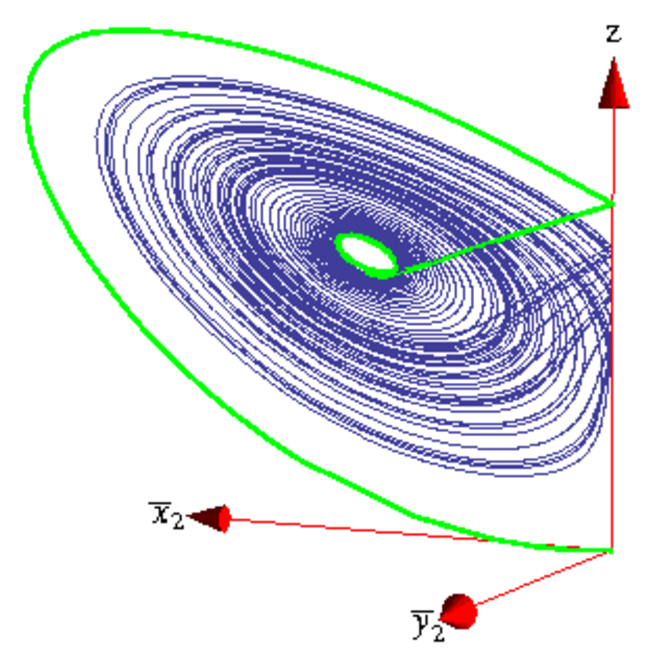
\includegraphics[width=0.35\textwidth,clip=true]{../figs/CLEinvXYZ}
~~~~(\textit{b})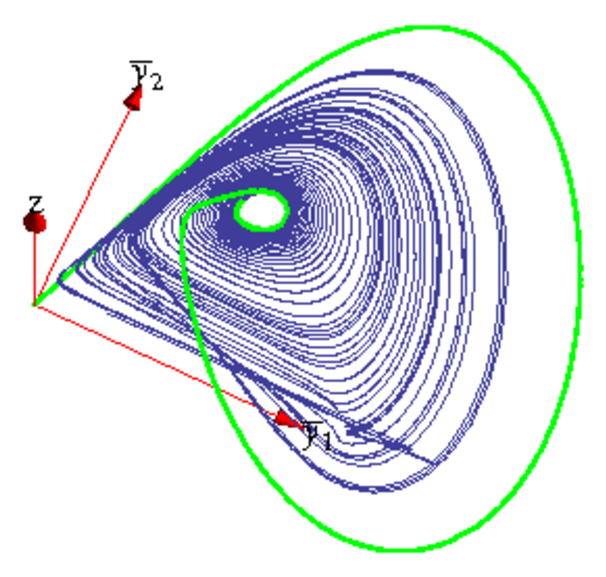
\includegraphics[width=0.35\textwidth,clip=true]{../figs/CLEinvYYZ}
\end{center}
\caption{
\Statesp\ portraits of \cLf\  in \reducedsp,
projected on invariant coordinates \refeq{eq:invLaser2}.
    }
\label{fig:CLEinv}
\end{figure}
%%%%%%%%%%%%%%%%%%%%%%%%%%%%%%%%%%%%%%%%%%%%%%%%%%%%%%%%%%%%%%%%
\ES{Fetch return map figure using unmodified invariants.}

%%%%%%%%%%%%%%%%%%%%%%%%%%%%%%%%%%%%%%%%%%%%%%%%%%%%%%%%%%%%%%%%%%
\begin{figure}[ht]
\begin{center}
%   (\textit{a})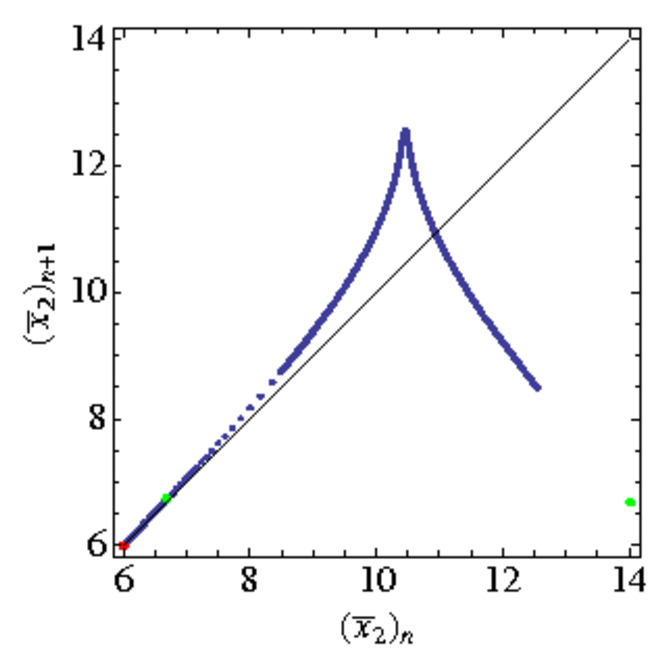
\includegraphics[width=0.35\textwidth,clip=true]{../figs/CLEinvRMx2}
%  ~~~~(\textit{b})
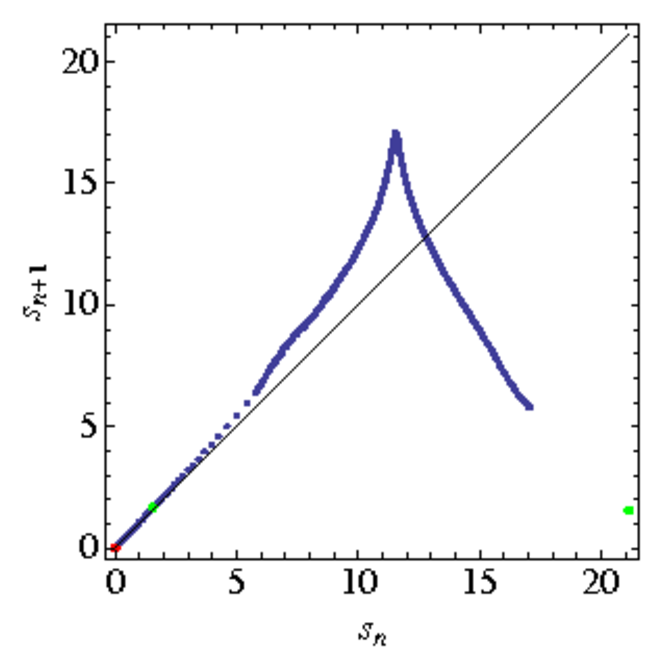
\includegraphics[width=0.35\textwidth,clip=true]{../figs/CLEinvRM}
\end{center}
\caption[Return map for Complex Lorenz flow]{
Return map to the \Poincare\ surface of section
$\overline{x}_2=\overline{y}_2$ for \cLe\ with $e=1/10$,
$\ImrCLor=0$, projecting on invariants given in
\refeq{eq:invLaser2}. The return map coordinate is the
Euclidean length along the \Poincare\ section of the unstable
manifold of $E_1$.
    }
\label{fig:CLEinvRM}
\end{figure}
%%%%%%%%%%%%%%%%%%%%%%%%%%%%%%%%%%%%%%%%%%%%%%%%%%%%%%%%%%%%%%%%

{\bf PC 2010-01-27:}
is the sign of the Lie algebra generator
\refeq{CLfLieGen}, group element standard?

{\bf ES 2010-01-28:}
    No. According
to Byron and Fuller, Mathematics of Classical and Quantum
Physics, which I find a very reliable and carefully written
book, what I use right now is the convention most physicists
use for \emph{active} transformations. This I've also used
in thesis and I'd be happy to stick with this. With this choice
small angle, active rotations, are counterclockwise, so I've updated
our orientation condition as well.

{\bf PC 2010-01-28:} Thanks, let's make sure that we have the
right sign in discrete.tex, continuous.tex (once CLE.tex is
submitted). Never seen Byron and Fuller.

{\bf ES 2010-01-28:}
A long time trajectory of \refeq{EqMotionMovFramePC} with
$\slicep$ on the \reqv\ \REQB{1} group orbit is shown in
\reffig{fig:CLEpcSect}.
As initial condition we chose an initial point on the unstable manifold
of \REQB{1}, rotated back to the \slice\ by angle $\theta$ as
prescribed by \refeq{PCsectQ1}.
    \PC{ in \reffig{fig:CLEpcSect}:\\
        * please, no both this figure and 'coincidentally'
          \reffig{fig:CLEmfReqb1}. \Mframes\ and \mslices\ are
          \emph{identical}, former is the integral version of the latter,
          so this is an embarrassing claim. The reduced flows are of course
          one and the same for the same choice of the slice point.
	  {\bf ES} Embarrassing indeed, did not come out right. My intention
	  was not to plot them at all and refer to \reffig{fig:CLEmfReqb1}.
	  But we do claim that with the integral
	  version we can ``pass'' through singularities, while with the differential
	  version they pose a real difficulty. So I want to let the reader know that
	  here we can obtain the same figure with both. Should this set of figures be omitted?
          \\
        * I think it is a bad idea too plot both $\{x_1,x_2,z\}$ and
          $\{y_1,y_2,z\}$ projections. They are too tightly coupled, and
          look very much the same. That is why in ChaosBook I plot
          $\{x_1,x_2,z\}$ and
          $\{x_1,y_2,z\}$ projections; the latter exhibits the sharp
          singular space discontinuity.
        * Mark $\ssp_{\REQB{}1}$ \\
        * Draw stable eigenvector of $\ssp_{\REQB{}1}$\\
        * State value of $\ssp_{\REQB{}1}$ somewhere
     {\bf ES:} Agreed. Draw stable eigenvector of $\ssp_{\REQB{}1}$? Not sure this would look
		  nice at this scale, I will instead indicate direction of motion along unstable
		manifold of \EQV{0} by arrow.}

{\bf PC 2010-01-29:} eliminated \reffig{fig:CLEmfssetOld}
from \reffig{fig:CLEmfsset}\,(b) and \reffig{fig:CLEmfAdHoc}\,(a).

%%%%%%%%%%%%%%%%%%%%%%%%%%%%%%%%%%%%%%%%%%%%%%%%%%%%%%%%%%%%%%%%
%computed with vaggelis/testing/flows/CLEfinalTmp.nb
\begin{figure}[ht]
\begin{center}
  (\textit{a})%kept \includegraphics[width=0.35\textwidth,clip=true]{../figs/CLEmfReqb123}
~~~~(\textit{b})\includegraphics[width=0.35\textwidth,clip=true]{../figs/CLEmfAdHoc123}
\end{center}
\caption{
\Statesp\ portraits of \cLf\ in \reducedsp. We use a
moving frame map to a slice orthogonal to the group tangent
at  (a) $\slicep  = \ssp_{\REQB{1}}$, (b) $\slicep  =
\ssp_{\REQB{1}}+(0,-5,0,0,0)$. The gray plane indicates the \sset.
    }\label{fig:CLEmfssetOld}
\end{figure}
%%%%%%%%%%%%%%%%%%%%%%%%%%%%%%%%%%%%%%%%%%%%%%%%%%%%%%%%%%%%%%%%

%%%%%%%%%%%%%%%%%%%%%%%%%%%%%%%%%%%%%%%%%%%%%%%%%%%%%%%%%%%%%%%%
%computed with vaggelis/testing/flows/CLEfinalTmp.nb
\begin{figure}[ht]
\begin{center}
  (\textit{a})\includegraphics[width=0.35\textwidth,clip=true]{../figs/CLEmfReqb135}
~~~~(\textit{b})% kept \includegraphics[width=0.35\textwidth,clip=true]{../figs/CLEmfAdHoc135}
\end{center}
\caption{
\Statesp\ portraits of \cLf\ in \reducedsp. We use a
moving frame map to a slice orthogonal to the group tangent
at  (a) $\slicep  = \ssp_{\REQB{1}}$, (b) $\slicep  =
\ssp_{\REQB{1}}+(0,-5,0,0,0)$. The shaded area indicates the \sset.
    }
\label{fig:CLEmfAdHoc}
\end{figure}
%%%%%%%%%%%%%%%%%%%%%%%%%%%%%%%%%%%%%%%%%%%%%%%%%%%%%%%%%%%%%%%%

%%%%%%%%%%%%%%%%%%%%%%%%%%%%%%%%%%%%%%%%%%%%%%%%%%%%%%%%%%%%%%%%
\begin{figure}[ht]
\begin{center}
  (\textit{a})% kept this 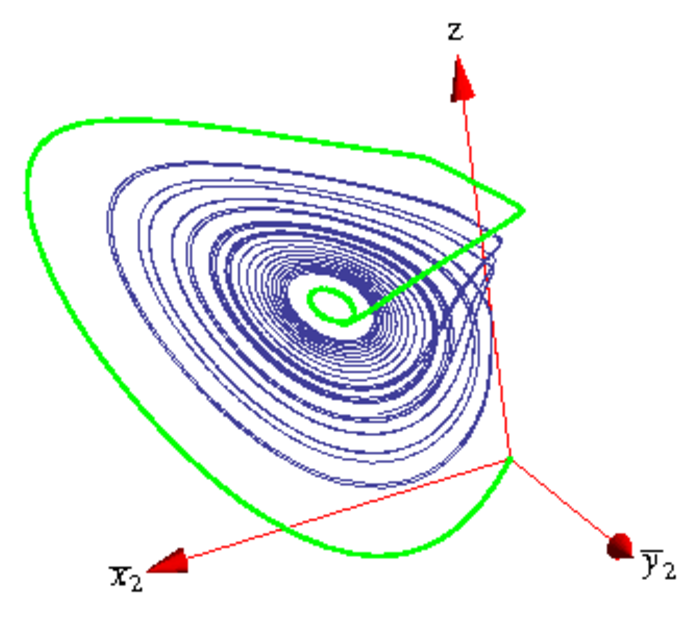
\includegraphics[width=0.35\textwidth,clip=true]{../figs/CLEmfXYZ}
 ~~~~(\textit{b})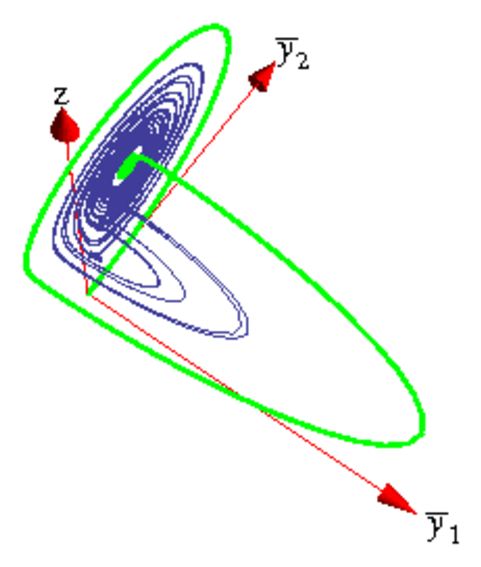
\includegraphics[width=0.35\textwidth,clip=true]{../figs/CLEmfYYZ}
\end{center}
\caption{
(a) \Statesp\ portrait of \cLf\ in \reducedsp,
projected on invariant coordinates  \refeq{eq:invLaser},
(b) The return map for the \Poincare\ surface of section $\sspRed_2=\sspRed_4$
for \cLe\ projected on invariant coordinates \refeq{eq:invLaser}.
The return map coordinate is the Euclidean length along the
\Poincare\ section of the unstable manifold of $\REQB{1}$.
    }
\label{fig:CLEmfOld}
\end{figure}
%%%%%%%%%%%%%%%%%%%%%%%%%%%%%%%%%%%%%%%%%%%%%%%%%%%%%%%%%%%%%%%%

%
%%%%%%%%%%%%%%%%%%%%%%%%%%%%%%%%%%%%%%%%%%%%%%%%%%%%%%%%%%%%%%%%
%computed with vaggelis/testing/flows/CLEfinalTmp.nb
\begin{figure}[ht]
\begin{center}
  (\textit{a})\includegraphics[width=0.35\textwidth,clip=true]{../figs/CLEperpReqb1}
~~~~(\textit{b}) % kept this: \includegraphics[width=0.35\textwidth,clip=true]{../figs/CLEperpReqb}
\end{center}
\caption{
\Statesp\ portraits of \cLf\ in \reducedsp. We use a
moving frame map to a slice orthogonal to the group tangent
at  $\slicep  = \ssp_{\REQB{1}}$.
    }
\label{fig:CLEmfReqb1}
\end{figure}
%%%%%%%%%%%%%%%%%%%%%%%%%%%%%%%%%%%%%%%%%%%%%%%%%%%%%%%%%%%%%%%%
%


% %%%%%%%%%%%%%%%%%%%%%%%%%%%%%%%%%%%%%%%%%%%%%%%%%%%%%%%%%%%%%%%%%%
% % computed in vaggelis/testing/flows/CLEfinalTmp.nb
% \begin{figure}[ht]
% \begin{center}
%  (\textit{a})\includegraphics[width=0.43\textwidth,clip=true]{CLEperpReqb1}
% ~(\textit{b}) \includegraphics[width=0.43\textwidth,clip=true]{CLEperpReqb}
% \end{center}
% \caption{
% \Statesp\ portraits of \cLf\  in \reducedsp\
% obtained by {\Mframes}, \slice\ fixed by a point on the
% \reqv\ group orbit, $\slicep  = \ssp_{\REQB{1}}$.
% (a) $\{x_1,x_2,z\}$ projection,
% (b) $\{y_1,y_2,z\}$ projection.
% }
% \label{fig:CLEpcSect}
% \end{figure}
% %%%%%%%%%%%%%%%%%%%%%%%%%%%%%%%%%%%%%%%%%%%%%%%%%%%%%%%%%%%%%%%%
%

% \PublicPrivate{}{
% % %%%%%%%%%%%%%%%%%%%%%%%%%%%%%%%%%%%%%%%%%%%%%%%%%%
% % % computed by PCunrot.nb
% % \SFIG{PCunrot1}
% % {}{
% % {\Mframes}, continuous time version, for the
% % polar coordinates motivated $x^{*}=(0,1,0,0)$,
% % $x_1=0,\;x_2>0$, \slice. The \cLf\ strange attractor of
% % \reffig{fig:CLE} exhibits a discontinuity at
% % $x_2=0$ in the \reducedsp:
% % $\{x_2,y_2,z\}$ projection.
% % }
% % {fig:PCunrot1}
% % %%%%%%%%%%%%%%%%%%%%%%%%%%%%%%%%%%%%%%%%%%%%%%%%%%
%
% Indeed, the method does encounter singularities in
% subsets of \statesp.
% For example, the \reducedsp\ equations \refeq{PCsectSin}
% for the polar coordinates inspired \slice\
% $x^{*}=(0,1,0,0)$, $x_1=0,\;x_2>0$,
% %this is illustrated by \reffig{fig:PCunrot}.
% %$(\rho_1,\theta_1)$ are polar coordinates, $\rho_1 =
% %\sqrt{\ssp_1^{ 2} + \ssp_2^{2}}$, see \refeq{eq:CartToPol},
% are given by
% \beq
% \dot{\ssp} = \vel - \frac{\vel_1}{\ssp_2} \Lg \cdot \ssp
% \,.
% \ee{EqMotionMovFrame}
% A typical trajectory is shown in \reffig{fig:PCunrot}.
%    \PC{this is not \reffig{fig:PCunrot} - copy correct fig
%        from wilczak/blog
%        }
% }

%\renewcommand{\Group}{\ensuremath{\Gamma}}    % Siminos Lie group

{\bf PC 2010-01-29:} replaced these two by their sum:
\beq
\left(
\begin{array}{c}
\dot{\theta}_1\\
\dot{\theta}_2
\end{array}
\right)
=
\left(
\begin{array}{c}
-\sigma\frac{r_2}{r_1}\sin\theta  \\
 e + (\rho_1-z)\frac{r_1}{r_2}\sin\theta
\end{array}
\right)
\,.
\label{eq:PolarCLeAnglesOld}
\eeq

{\bf PC 2010-01-29 replaced by ChaosBook.org version:}

\beq
\begin{split}
\dot{\overline{x}}_1 &= 0\,\\
\dot{\overline{x}}_2 &=-\sigma  \left(\overline{x}_2-\overline{y}_2 \right)\,,\\
\dot{\overline{y}}_1 &=-\overline{y}_1- \left(e+\sigma\frac{\overline{y}_1}{\overline{x}_2} \right)\overline{y}_2\,,\\
\dot{\overline{y}}_2 &=(\RerCLor -z)\overline{x}_2+\left(e+\frac{\sigma  \overline{y}_1}{\overline{x}_2}
\right) \overline{y}_1-\overline{y}_2\,,\\
\dot{z} &=\overline{x}_2 \overline{y}_2-b z\,.
\end{split}
\eeq

{\bf PC 2010-01-29 dropped:}

    Looks like one should also read \refref{Abraham95}; they
    report on various return maps.

   explain that we have used ``
$\Lg_a{}^T \Lg_b = \sum_\alpha C_2^{(\alpha)} \delta_{ab} \, \id^{(\alpha)}$
    ''

    {\bf ES:} I've updated figure \reffig{fig:CLEmfAdHoc}
	to compare $(x_1,y_1,z)$ projection with the two different choices.
	I'm not sure that the plot of the singular set is accurate in this
	projection though. To me the difference is clear here, the image
	system in the second case is as smooth as with in\-vari\-ant polynomials.
    {\bf PC} I combined the two figures, removed \reffig{fig:CLEmfAdHoc}.
     There is
     no need to say "a slice orthogonal to the group tangent". For our
     linear slices it is so by construction.

dropped CLEip2.eps, svn mv it to OldFig. ({\bf ES} This would
     break thesis.)
    CLEip1 was plotted by the devil, it is cool 2MB.

    {\bf PC} I think this is wrong, safer to drop it:
``In the \cLe\ example no
trajectories enter the $x_1=x_2=0$ subspace, but this is a
fortuitous event'' so I am dropping it. Without any loss of
information. {\bf ES} Do you think that generic trajectories do enter $x_1=x_2=0$
or that it is not a fortuitous event? I am also confused so it's
better to drop it.

    \PublicPrivate{.}{ % switch to private
(see \reffig{fig:GrpOrbTang}).
    }% end \PublicPrivate

{\ES dropped text from stability appendix:}

Using the {\mframes} to map dynamics on a slice $\pSRed$ as
in \refsect{sec:mf} or restricting integration on the slice
as in \refsect{sec:MovFrameODE}, the reduced \statesp\ is
identified (at least locally) with the {\slice} ${\pSRed}$.
This provides a means of calculating stability of \reqva\ in
reduced \statesp. Proof that such a notion of stability of
\reqva\ is meaningful is given, for instance, in
\refref{Krupa90}.  To simplify notation we only treat
the one-dimensional group case and drop all group parameter
related indices, writing $\Lg_{ij}$ instead of
$(\Lg_1)_{ij}$, \etc.
    \ES{To Predrag: I couldn't find Chossat and Lauterbach book
    here. If you have it would it be easy to have a look at their
    expression for stability of \reqva? Is this claim correct? I
    remember that my motivation to derive it was that their
    expression is too implicit to use in practice, while Krupa's
    is totally abstract. But maybe I was missing something.
    {\bf PC:} no time for me to go to the library now
    and check this...
    }
    \PC{the problem is that this formula is based on
    the \emph{method of connections} of Rowley
    \etal\rf{rowley_reduction_2003} which we cannot use
    because its additional \emph{geometric phase}. They prove
    a theorem
    - as well as probably Beyn - that it is OK for \reqva.
    {\bf ES:} Yes, this is why we only use it for stability of \reqva.
	      I will have to try rpo stability using projection we use
	      for integration on the slice, but it is too late for this paper.
	      I had the well known problem back then, I did not understand
	      derivation of Rowley and Marsden.
    }

In \ref{s:StabReq} we derive an expression for the stability
of \reqva\ (traveling waves) in \reducedsp\
that can be applied without an explicit
calculation of the reduced system.
    \PC{unless you clean up \ref{s:StabReq} now, it will have to
        be omitted.}

\section{\label{s:StabReq} Stability of \reqva}
        \PC{this appendix does not seem ready for the prime time.
        If we refer to it as in the above 'Public' version you
        will have to update your thesis.
        }
%     \input stabReqva



    } %end \PublicPrivate{%

\end{document}
